%%%%%%%%%%%%%%%%%%%%%%%%%%%%%%%%%%%%%%%%%
% Stylish Article
% LaTeX Template
% Version 2.1 (1/10/15)
%
% This template has been downloaded from:
% http://www.LaTeXTemplates.com
%
% Original author:
% Mathias Legrand (legrand.mathias@gmail.com) 
% With extensive modifications by:
% Vel (vel@latextemplates.com)
%
% License:
% CC BY-NC-SA 3.0 (http://creativecommons.org/licenses/by-nc-sa/3.0/)
%
%%%%%%%%%%%%%%%%%%%%%%%%%%%%%%%%%%%%%%%%%

%----------------------------------------------------------------------------------------
%       PACKAGES AND OTHER DOCUMENT CONFIGURATIONS
%----------------------------------------------------------------------------------------

\documentclass[fleqn,10pt]{SelfArx} % Document font size and equations flushed left
\usepackage[english]{babel} % Specify a different language here - english by default
\usepackage{lipsum} % Required to insert dummy text. To be removed otherwise
\usepackage{url} % Required to insert dummy text. To be removed otherwise
\usepackage{balance}

\usepackage{hyperref}
\usepackage{mathptmx}
\usepackage{times}
\usepackage{textcomp}
\usepackage{gensymb} % degree. ie 360º
\usepackage{amsmath}
\usepackage{comment}
\usepackage{multirow}
\usepackage[framemethod=tikz]{mdframed}
\usepackage{graphicx}
\usepackage[labelfont=bf]{subcaption}
\usepackage{eucal}

%------------------------------------------------------------------------------
\usepackage{ifthen}

\newboolean{draft}
\setboolean{draft}{true}

%------------------------------------------------------------------------------
\usepackage[T1]{fontenc}
\usepackage{adjustbox}
\usepackage{url}
\usepackage[utf8]{inputenc}
\usepackage{verbatim}
\usepackage{amsmath,amsfonts,amsthm}
\usepackage{caption}
\usepackage{graphicx}
\usepackage{framed}
\usepackage{mathtools}
\usepackage{ragged2e}
\usepackage{cancel}
%\usepackage[a4paper]{geometry}
\usepackage{multirow}
\usepackage{rotating}
\usepackage{graphicx}
\usepackage{float}
\usepackage{booktabs}
\usepackage{color}

%------------------------------------------------------------------------------
\usepackage{tikz}
\usetikzlibrary{arrows,positioning}
\usetikzlibrary{shapes}
\usetikzlibrary{patterns}

%------------------------------------------------------------------------------
\usepackage[ruled]{algorithm2e}

\SetKwFor{For}{For}{}{}
\SetKwFor{While}{While}{}{}
\SetKwRepeat{Do}{Do}{while}
\SetKwIF{If}{IfElse}{Else}{If}{}{Else if}{Else}{}
\SetKw{Return}{Return}
\SetKwInput{Input}{Input}

%------------------------------------------------------------------------------
\usepackage[colorinlistoftodos,portuguese]{todonotes}

\newcommand{\rc}[1]{
	\ifthenelse{\boolean{draft}}{
		{
			\linespread{0.8}
			\todo[color=yellow!40,linecolor=red]{#1}}\linespread{1.5}
	}
	{}
}

\newcommand{\alane}[1]{
	\ifthenelse{\boolean{draft}}{
		{
			\linespread{0.8}
			\todo[color=blue!10,linecolor=blue]{#1}}\linespread{1.5}
	}
	{}
}

\newcommand{\Problema}[3]{
	\begin{algorithm}[h]
		\NoCaptionOfAlgo
		\caption{#1}
		\SetKwInOut{Input}{Instance}
		\SetKwInOut{Output}{Answer}
		
		\Input{#2}
		
		\Output{#3}
	\end{algorithm}
}

%------------------------------------------------------------------------------
\DeclarePairedDelimiter\ceil{\lceil}{\rceil}
\DeclarePairedDelimiter\floor{\lfloor}{\rfloor}

\newtheorem{teor}{Theorem}
\newtheorem{lema}{Lemma}
\newtheorem{defin}{Definition}

\newcommand{\NP}{\ensuremath{\mathcal{N}\mathcal{P}}}
\newcommand{\bI}{\textbf{I}}

\newcommand{\chaves}[1] {\ensuremath{{\left \{ {#1} \right \}}}}
\newcommand{\parenteses}[1] {\ensuremath{\left ( {#1} \right )}}
\newcommand{\Min}[1] {\ensuremath{\min\chaves{#1}}}
\newcommand{\Max}[1] {\ensuremath{\max\chaves{#1}}}

\newcommand{\cC}{\mathcal{C}}
\newcommand{\cO}{\mathcal{O}}

\newcommand{\bN}{\ensuremath{\mathbb{N}}}

\newcommand{\pordef}{\ensuremath{\mathrel{:\mkern-0.25mu=}}}

%\raggedbottom



\usepackage{tcolorbox}% http://ctan.org/pkg/tcolorbox
\definecolor{mycolor}{rgb}{0,0,0}% Rule colour
\makeatletter
\newcommand{\mybox}[1]{%
	\setbox0=\hbox{#1}%
	\setlength{\@tempdima}{\dimexpr\wd0+13pt}%
	\begin{tcolorbox}[colframe=mycolor,boxrule=0.5pt,arc=4pt,
		left=6pt,right=6pt,top=6pt,bottom=6pt,boxsep=0pt,width=\@tempdima]
		#1
	\end{tcolorbox}
}
\makeatother
\usepackage[resetlabels,labeled]{multibib}
\newcites{A}{Appendix}
\usepackage[num]{abntex2cite}
\citebrackets[]
%----------------------------------------------------------------------------------------
%       COLUMNS
%----------------------------------------------------------------------------------------
\setlength{\columnsep}{0.55cm} % Distance between the two columns of text
\setlength{\fboxrule}{0.75pt} % Width of the border around the abstract
%----------------------------------------------------------------------------------------
%       COLORS
%----------------------------------------------------------------------------------------
\definecolor{color1}{RGB}{0,0,90} % Color of the article title and sections
\definecolor{color2}{RGB}{0,20,20} % Color of the boxes behind the abstract and headings
%----------------------------------------------------------------------------------------
%       HYPERLINKS
%----------------------------------------------------------------------------------------
\usepackage{hyperref} % Required for hyperlinks
\hypersetup{hidelinks,colorlinks,breaklinks=true,urlcolor=color2,citecolor=color1,linkcolor=color1,bookmarksopen=false,pdftitle={Title},pdfauthor={Author}}
%----------------------------------------------------------------------------------------
%       ARTICLE INFORMATION
%----------------------------------------------------------------------------------------

\JournalInfo{\color{gray}\normalsize\sffamily\bfseries Revista de Informática Teórica e Aplicada - RITA - ISSN 2175-2745\\ Vol.~25, Num.~04~(2018)~57-73} % Journal information
\Archive{\mybox{RESEARCH ARTICLE}} % Type of Article: Researh, Review, Tutorial, Study Case

\PaperTitle{Exact Algorithms for the Graph Coloring Problem} % Article title - English

\ShortTitle{Exact Algorithms for the Graph Coloring Problem} % Short Article title - English

\Titulo{Algoritmos Exatos para o Problema da Coloração de Grafos} % Article title - Portuguese

\PaperVol{25} % Volume 
\PaperNum{4} % Number 
\PaperAno{2018} % Year of Publication


\Authors{Alane Marie de Lima\textsuperscript{1}*, Renato Carmo\textsuperscript{2}} % Authors
\affiliation{\textsuperscript{1,2}\textit{Informatics, Federal University of Parana, Brazil}} % Author affiliation
%\affiliation{\textsuperscript{2}\textit{Informatics, Federal University of Parana, Brazil}} % Author affiliation
\affiliation{*\textbf{Corresponding author}: amlima@inf.ufpr.br} % Corresponding author




\Keywords{Graph Theory --- Graph Coloring --- Exact Algorithms}

\newcommand{\keywordname}{Keywords} % Defines the keywords heading name

\PalavrasChave{Teoria dos Grafos --- Coloração de Grafos --- Algoritmos Exatos} 


\Doi{https://doi.org/10.22456/2175-2745.80721} % DOI
\DateR{01/03/2018} % Received
\DateA{05/06/2018} % Accepted

%----------------------------------------------------------------------------------------
%       ABSTRACT
%----------------------------------------------------------------------------------------

\Abstract{The graph coloring problem is the problem of partitioning the vertices of a graph into the smallest possible set of independent
	sets. Since it is a well-known NP-Hard problem, it is of great interest of the computer science finding results over exact algorithms that solve it. The main algorithms of this kind, though, are scattered through the literature. In this paper, we group and contextualize some of these algorithms, which are based in Dynamic Programming, Branch-and-Bound and Integer Linear Programming. The algorithms for the first group are based in the work of Lawler, which searches maximal independent sets on each subset of vertices of a graph as the base of his algorithm. In the second group, the algorithms are based in the work of Brelaz, which adapted the DSATUR procedure to an exact version, and in the work of Zykov, which introduced the definition of Zykov trees. The third group contains the algorithms based in the work of Mehrotra and Trick, which uses the Column Generation method.\\}

\Resumo{O problema de coloração de grafos consiste em
	particionar os vértices de um grafo na menor quantidade
	possível de conjuntos independentes. Por tratar-se de um
	problema NP-Difícil conhecido, é de grande interesse da
	computação encontrar resultados sobre algoritmos exatos para sua
	solução. Entretanto, os principais dentre estes algoritmos
	estão espalhados pela literatura. Neste artigo, agrupamos e
	contextualizamos alguns destes algoritmos, a saber, soluções
	baseadas em Programação Dinâmica, Branch-and-Bound e
	Programação Linear Inteira. Os algoritmos do primeiro grupo
	são baseados no trabalho de Lawler, que busca conjuntos
	independentes maximais em cada subconjunto de vértices de um
	grafo como base de seu algoritmo. No segundo grupo, os
	algoritmos são baseados no trabalho de Brelaz, que adaptou a
	heurística DSATUR para uma versão exata, e no trabalho de
	Zykov, que introduziu o conceito de árvores de Zykov. O
	terceiro grupo contém algoritmos baseados no trabalho de
	Mehrotra e Trick, que utilizaram o método Geração de Colunas.\\}
%----------------------------------------------------------------------------------------

\begin{document}
	
	\setcounter{page}{57}
	
	\flushbottom % Makes all text pages the same height
	\maketitle % Print the title and abstract box
	\thispagestyle{empty} % Removes page numbering from the first page
	%\tableofcontents % Print the contents section
	
	
	%----------------------------------------------------------------------------------------
	%       ARTICLE CONTENTS
	%----------------------------------------------------------------------------------------
	
	
	
	\section{Introduction} % The \section*{} command stops section numbering
	
	\addcontentsline{toc}{section}{Introduction} % Adds this section to the table of contents
	Graph coloring is the problem of assigning colors to the vertices of a graph in
	such a way that neighbor vertices are assigned with different colors. The
	problem of coloring a graph with the minimum possible number of colors
	is a fundamental \NP-Hard problem with a number of applications of
	interest such as timetabling, code optimization and seating plans \cite{Lewis2015}.
	
	Information on different approaches for this and related computational
	problems are scattered throughout the literature. We survey some of
	these approaches discussing their strengths and weaknesses.
	
	The algorithms we discuss are based on three main approaches, namely,
	Dynamic Programming, Branch-and-Bound and Linear Programming. Besides
	these, we also discuss the \textsf{DSATUR} algorithm for graph
	coloring.
	
	The text is organized as follows. In Section~\ref{sec:defs} we briefly
	state some definitions and the notation used. Section~\ref{sec:dyn}
	discusses algorithms based in Dynamic
	Programming. Section~\ref{sec:bb} discusses algorithms based in
	Branch-and-Bound. Section~\ref{sec:lp} discusses algorithms based in
	Linear Programming. Finally, Section~\ref{sec:conclusion} contains the
	conclusions.
	
	%..............................................................................
	\subsection{Definitions and Notation}\label{sec:defs}
	
	Given a set $S$ and an integer $k$, we denote by $\binom{S}{k}$ the
	set of subsets of $S$ of size $k$.
	
	A graph $G$ is a pair $(V(G),E(G))$ where $V(G)$ is a finite set (the
	vertices of $G$) and $E(G) \subseteq \binom{V(G)}{2}$ (the edges of
	$G$). Note that, according to these definitions, graphs in this text
	are simple, that is, have no multiple edges or loops.
	
	Two vertices $u$ and $v$ are \emph{neighbors} in $G$ if
	$\chaves{u,v} \in E(G)$.  The \emph{degree} of vertex $v$ in $G$ is the
	number of neighbors of $v$ in $G$ and is denoted by $d_G(v)$.
	
	The induced subgraph of $G$ by a set $S \subseteq V(G)$ is
	denoted by $G[S]$ and the graph $G-S$ is the graph $G[V(G)-S]$. If
	$v \in V(G)$, we write $G-v$ instead of $G - \chaves{v}$.  
	
	The set $S \subset V(G)$ is \emph{independent} in $G$ if no vertices in
	$S$ are neighbors in $G$ and is a \emph{maximal independent set} in
	$G$ if it is not properly contained in another independent set in $G$.
	We denote by $\bI(G)$ the set of all maximal independent sets in $G$.
	
	Given an integer $k \leq |V(G)|$, a \emph{$k$-coloring} of $G$ is a
	partition of $V(G)$ into
	$k$ independent sets in $G$. Each such set is called a \emph{color} in
	the coloring. A graph $G$ is $k$-colorable if it admits a
	$k$-coloring. The smallest $k$ for which $G$ is $k$-colorable called
	the \emph{chromatic number} of $G$ and is denoted $\chi(G)$. An
	\emph{optimal coloring} of $G$ is a $\chi(G)$--coloring of $G$.
	
	%..............................................................................
	\subsection{Graph Coloring Problems}\label{sec:complexity}
	
	We define the following $\NP$-Hard problems:
	
	\Problema{Graph Coloring}{a graph $G$}{a $\chi(G)$-coloring of $G$}
	\Problema{Chromatic Number}{a graph $G$}{$\chi(G)$}
	\Problema{$k$-coloring}{a graph $G$ and $k \in \bN$}{YES, if we can color $G$ with no more than $k$ colors; NO, otherwise.}
	
	Graph coloring problems are polynomially solvable when the given graph $G$ is 2-colorable. The problems are also efficiently solvable for some graph classes, where we highlight here the perfect graphs \cite{Grotschel84}.
	
	%------------------------------------------------------------------------------
	\section{Dynamic Programming Algorithms}\label{sec:dyn}
	
	In this section, we discuss dynamic programming algorithms for the
	graph coloring problem. Dynamic Programming is the approach of
	computing the answer to an instance of a problem by computing and
	combining the answers to ``sub-instances'' of that instance (see, for
	example,~\cite[chapter 15]{CormenLeisersonRivestStein09}).
	
	We start with an algorithm from Lawler~\cite{Lawler76} (Section~\ref{sec:lawler}) which has $\cO^*(2.4423^n)$ running
	time. Then we discuss an algorithm from Eppstein~\cite{Eppstein03}
	(Section~\ref{sec:eppstein}) which, through a modification of the idea
	of Lawler's algorithm, improves this bound to
	$\cO(2.4150^n)$. Next (Section~\ref{sec:byskov}), we discuss a
	modification of Eppstein's algorithm in Byskov~\cite{Byskov03} yielding
	an $\cO(2.4023^n)$ algorithm. 
	
	All the above algorithms require exponential space. In
	Section~\ref{sec:bodlaender-kratsch} we discuss an
	$\cO(5.283^n)$ running time algorithm
	from Bodlaender and Kratsch~\cite{BodlaenderKratsch06} requiring polynomial space.
	
	Unless otherwise stated, the proofs of the results in
	sections~\ref{sec:lawler},~\ref{sec:eppstein} and~\ref{sec:byskov} are
	based on those in~\cite{Byskov03}.
	
	%..............................................................................
	\subsection{Lawler's Algorithm}\label{sec:lawler}
	
	Lawler\cite{Lawler76} was the first to propose a dynamic programming
	algorithm for the graph coloring problem, as described in Algorithm 4. One may view his algorithm as based in the following result.
	
	\begin{teor}[Wang\cite{Wang1974}]\label{teo:wang} 
		Every graph has an optimal coloring in which (at least) one of the
		colors is a maximal independent set.
	\end{teor}
	\begin{proof}
		Let $\cC = \chaves{P_1, \ldots,P_k}$ be an optimal coloring of $G$ and
		let $I$ be a maximal independent set containing $P_{1}$. Then
		$\chaves{I, P_2 \setminus I, \ldots,P_k \setminus I}$ is an optimal coloring of
		$G$ and one of its colors is a maximal independent set.
	\end{proof}
	
	It follows from Theorem~\ref{teo:wang} that if $G$ is a graph and
	$S \subseteq V(G)$, then $\chi(G[S])$ is the
	minimum among $1+\chi(G[S\setminus{}I])$ over all maximal independent sets
	$I$ in $G[S]$, that is,
	\begin{equation*}
	\chi(G[S])
	=
	\begin{cases}
	0, & \text{if } S = \emptyset, \\
	1 + \Min{\chi(G[S \setminus I])\colon I \in \bI(G[S])}, & \text{otherwise}.
	\end{cases}
	\end{equation*}
	
	\begin{algorithm}[h]\label{alg:lawler}
		\SetAlgoNoLine
		\DontPrintSemicolon
		\KwIn{A graph $G$}
		\KwResult{The chromatic number of $G$}
		
		$n \gets |V(G)|$ \;
		
		$X \gets$ array indexed from $0$ to $2^{n}-1$ \;
		
		$X[0] \gets 0$ \;
		
		\For{$S \gets 1 \text{ to } 2^n-1$}{ 
			
			$s \gets f(S)$ \;
			
			$X[s] \gets \infty$ \;
			
			\For{$I \in \bI(G[S])$}{
				
				$i \gets f(S \setminus I)$ \;
				
				\If{$X[i]+1 < X[s]$}{
					
					$X[s] \gets X[i]+1$
				}
			}
		}
		
		\Return{$X[2^n-1]$}
		\caption{\textsc{Lawler$(G)$}}
	\end{algorithm}
	
	For each $S \subseteq V(G)$, the chromatic number of $G[S]$  is stored in 
	$X[f(S)]$. The function $f\colon 2^{|V(G)|} \to \chaves{0, \ldots, 2^{n}-1}$
	indexes the subsets of $V(G)$ in such a way that $f(X) < f(S)$ for all
	$X \subset S$ (for instance, by returning $f(S) = \sum_{v_i \in S} 2^i - 1$, where
	$V(G) = \chaves{v_{0}, \ldots, v_{n-1}}$ is an ordering of $V(G)$).
	
	It should be noted that the inner loop in Algorithm~4
	performs a non-trivial task, namely, enumerating all maximal
	independent sets of a graph. As Lawler~\cite{Lawler76} itself notes,
	this can be done in time $\cO(n m I)$ for a graph with $n$ vertices,
	$m$ edges and $I$ maximal independent subsets~\cite{Tsukiyama77}.
	
	\begin{teor}\label{teo:lawler} 
		Algorithm~4 runs in time
		$\cO(2.4423^n n m)$ and space $\Theta(2^n)$, if the input is a
		graph with $n$ vertices and $m$ edges.
	\end{teor}
	\begin{proof} 
		Let $G$ be a graph with $n$ vertices and $m$ edges. For
		each $S \subseteq V(G)$, let $T(S)$ denote the time spent in the execution
		of the inner loop in Algorithm~4 using the
		algorithm from Tsukiyama\cite{Tsukiyama77}. Then we know that there
		exist $c > 0$ and $n_{0} \in \bN$ such that, whenever $|S| \geq
		n_{0}$, 
		\begin{equation*}
		T(S) \leq c\, |S|\, |E(G[S])|\, |\bI(G(S))| \leq c n m 3^{|S|/3},
		\end{equation*}
		because a graph on $k$ vertices can have at most $3^{k/3}$ maximal
		independent sets~\cite{MoonMoser65}.
		
		Summing over all $S \subseteq V(G)$ we get
		\begin{multline*}
		\sum_{S \subseteq V(G)} T(S)
		\leq
		\sum_{S \subseteq V(G)} c n m 3^{|S|/3}
		=
		c n m \sum_{S \subseteq V(G)} 3^{|S|/3} \\
		=
		c n m \sum_{i=0}^{n} \sum_{S \in \binom{V(G)}{i}} 3^{|S|/3} 
		=
		c n m \sum_{i=0}^{n} \sum_{S \in \binom{V(G)}{i}} 3^{i/3} \\
		=
		c n m \sum_{i=0}^{n} \binom{n}{i} 3^{i/3} 
		=
		c n m \sum_{i=0}^{n} \binom{n}{i} \parenteses{3^{1/3}}^{i} \\
		\leq
		c n m \parenteses{1+3^{1/3}}^{n}
		\leq 
		c n m \parenteses{2.4423}^{n}.
		\end{multline*}
		
		Hence we can conclude that the execution time of
		Algorithm~4 with $G$ as input is
		$\cO(n m \parenteses{2.4423}^{n})$.
	\end{proof}
	
	%..............................................................................
	\subsection{Eppstein's Algorithm}\label{sec:eppstein}
	
	Lawler's algorithm (Algorithm 4) had the best upper bounds for the graph coloring
	problem until Eppstein~\cite{Eppstein03} proposed two modifications.  The
	first one is the preprocessing of the $3$-colorable subgraphs of the
	input graph. The other one is filling in vector $X$ (the dynamic
	processing table) in a different order which allows for skipping the
	processing of maximal independent sets beyond a certain size.
	
	Let us start with the following result.
	
	\begin{teor}[Madsen, Nielsen and Skjernaa~\cite{MadsenNielsenSkjernaa02}]\label{teo:mns} 
		Let $G$ be a graph and let $J' \subseteq V(G)$ be such that $G[J']$ is a
		maximal $k$-colorable subgraph of $G$. For every $0 \leq k_1 < k$ there
		is a set $J \subseteq J'$ such that $G[J]$ is a maximal
		$k_1$-colorable subgraph of $G[J']$ and $G[J' \setminus J]$ is a maximal
		$(k-k_1)$-colorable subgraph of $G-J$.
	\end{teor}
	\begin{proof}   

		Let $G$ be a graph and let
		$J' \subseteq V(G)$ be such that $G[J']$ is a maximal
		$k$-colorable subgraph of $G$. Given $k_{1} \leq k$, let
		$\chaves{I_{1}, \ldots, I_{k}}$ be an optimal coloring of $G[J']$ in such a
		way that $|I_{1}| \geq |I_{2}| \geq \ldots \geq |I_{k}|$ and 
		$J \pordef \bigcup_{i=1}^{k_{1}} I_i$ is the largest
		possible.  Then $G[J]$ is a maximal $k_1$-colorable subgraph of
		$G[J']$.
		Because $G[J']$ is maximal, there can be no vertex
		$v \in V(G) \setminus J'$ that can be added either to $G[J]$ or to
		$G[J' \setminus J]$ so that $G[J' \cup \chaves{v}]$ remains
		$k$-colorable.
		Hence, $G[J' \setminus J]$ is a maximal $(k-k_1)$-colorable subgraph in
		$G-J$.

	\end{proof}
	
	It is possible to prove (see \cite[sec. 3.2.2]{Lima17}) that if $k_1 = k-1$ then $G[J' \setminus J]$ is a maximal independent set in $G-J$. The proof is
	similar to the one of Theorem~\ref{teo:mns} with the chosen optimal
	coloring being one in which $I_k$ has the smallest possible size.
	
	From Theorem~\ref{teo:mns}, we have that if $G[J']$ is a maximal
	$k$-colorable subgraph of $G$, then it has an optimal coloring $\chaves{I_{1}, \ldots, I_{k}}$ such that $I_k$ has the smallest
	size as possible. Then we have a set $J$ such that
	$J = J' \setminus I_k$ and $G[J]$ is $(k-1)$-colorable. The same way as
	$G[J']$, the graph $G[J]$ has a color $I_{k-1}$ in one of its
	optimal colorings such that $I_{k-1}$ has the smallest size as
	possible. Hence,
	\begin{equation*}
	|J| 
	=
	\sum_{i=1}^{\chi(G[J])} |I_i| 
	\geq 
	\sum_{i=1}^{\chi(G[J])} |I_{k-1}| 
	=
	|I_{k-1}|\chi(G[J])
	\end{equation*}
	
	Since $|I_k| \leq |I_{k-1}|$, then $|I_k| \leq
	|J|/\chi(G[J])$. Hence, for each $S \subseteq V(G)$, the value of $\chi(G[S \cup~ I])$ is the minimum among $1+\chi(G[S])$ over all maximal independent sets $I \leq |S|/\chi(G[S])$, that is, 
	\begin{small}
	\begin{equation*}
	\chi(G[S \cup I]): I \in {\bf I}(G-S)
	=
	\begin{cases}
	0, & \text{if } S \cup I = \emptyset, \\
	1 + \Min{\chi(G[S])}, & \text{otherwise}.
	\end{cases}
	\end{equation*}
	\end{small}
	% In this Section, we show the algorithms of Eppstein for finding the
	% chromatic number and the optimal coloring of a graph, described in
	% Algorithms~\ref{alg:2} and \ref{alg:optc}, respectively. We also
	% introduce the $3$-coloring algorithm used in the stage of
	% pre-processing.
		
	The chromatic number of $G[S]$ is stored in $X[f(S)]$, for each $S \subseteq V(G)$. The function $f(S)$ is the one defined in Section~\ref{sec:lawler}.
	The function $c(S)$ associates each $S$ to its corresponding graph $G[S]$. 
	
	\begin{algorithm}[h]
		\SetAlgoNoLine
		\KwIn{A graph $G$}
		\KwResult{The chromatic number of $G$}
		%\Inicio{
		$n \gets |V(G)|$\\
		$X \gets$ array indexed from 0 to $2^n-1$\\
		$X[0] \gets 0$ \\
		\For{$S \gets 1 \text{ to } 2^n-1$}{
			$i \gets f(S)$\\
			Run the algorithm of Beigel and Eppstein~\cite{BeigelEppstein05} in $G[S]$.\\
			\If{$\chi(G[c(S)]) \leq 3$}{
				$X[i] \gets \chi(G[c(S)])$
			}\Else{
				$X[i] \gets \infty$
			}
		}
		
		\For{$S\gets1 \text{ to } 2^n-1$}{
			$i \gets f(S)$\\
			\If{$3 \leq X[i] < \infty$}{
				\For{$I \in \bI(G-S)$ such that $|I| \leq |S|/X[S]$}{
					$j \gets f(S \cup I)$\\
					\If{$X[i]+1 < X[j]$}{
						$X[j] \gets X[i]+1$
					}                     
				}
			}
		}
		%}
		\Return{$X[2^n-1]$}
		\caption{\textsc{Eppstein$(G)$}}\label{alg:2}
	\end{algorithm}
	
	\begin{teor}Algorithm 5 runs in time
		$\cO(2.4150^n)$ and space $\cO(2^n)$. \label{teo:epps}
	\end{teor}
	
	\begin{proof}
		
		Let $G$ be a graph with $n$ vertices and $m$ edges. For
		each $S \subseteq V(G)$, let $T(S)$ denote the time spent in the preprocessing of the 3-colorable subgraphs using the algorithm from Beigel and Eppstein\cite{BeigelEppstein05}, which runs in $\cO(1.3289^n)$. Then we know that there
		exist $c > 0$ and $n_{0} \in \bN$ such that, whenever $|S| \geq
		n_{0}$, 
		\begin{equation*}
		T(S) \leq c 1.3289^{|S|}
		\end{equation*}
		
		Summing over all $S \subseteq V(G)$ we get
		\begin{multline*}
		\sum_{S \subseteq V(G)} T(S)
		\leq
		\sum_{S \subseteq V(G)} c 1.3289^{|S|}
		=
		c \sum_{S \subseteq V(G)} 1.3289^{|S|} \\
		=
		c \sum_{i=0}^{n} \sum_{S \in \binom{V(G)}{i}} 1.3289^{|S|} 
		=
		c \sum_{i=0}^{n} \sum_{S \in \binom{V(G)}{i}} 1.3289^i \\
		=
		c \sum_{i=0}^{n} \binom{n}{i} 1.3289^i 
		\leq
		c \parenteses{1+1.3289}^{n} 
		\leq 
		c \parenteses{2.3289^n}.
		\end{multline*}
		
		Let $T'(S)$ be the time to process the maximal independent sets of size at most $k$ in $G[S]$, for $k \in \bN$. Then, there exist $c'>0$ and $n_1 \in \bN$ such that, whenever $|S| \geq n_1$, 
		
		\begin{multline*}
		\sum_{S \subseteq V(G)} T'(S)
		\leq
		\sum_{S \subseteq V(G)} c' 3^{\frac{4|S|}{3}-(n-|S|)}4^{(n-|S|)-3\frac{|S|}{3}} \\
		=
		c' \sum_{i=0}^{n} \sum_{S \in \binom{V(G)}{i}} 3^{\frac{4|S|}{3}-(n-|S|)}4^{(n-|S|)-3\frac{|S|}{3}} \\
		=
		c' \sum_{i=0}^{n} \sum_{S \in \binom{V(G)}{i}} 3^{\frac{4i}{3}-(n-i)}4^{(n-i)-3\frac{i}{3}} \\
		=
		c' \sum_{i=0}^{n} \binom{n}{i} 3^{\frac{7i}{3}-n}4^{n-2i} 
		\leq
		c' \parenteses{\frac{4}{3}}^n \parenteses{1+\frac{3^{\frac{7}{3}}}{4^2}}^{n} \\
		\leq 
		c' \parenteses{\frac{4}{3}+\frac{3^{4/3}}{4}}^{n}
		\leq
		c'(2.4150^n)
		\end{multline*}
		
		because the number of maximal independent sets of size at most $k$, for $k \in \bN$, is
		\begin{equation*}
		\floor{n/k}^{(\floor{n/k}+1)k-n}{(\floor{n/k}+1)}^{n-\floor{n/k}k}
		\end{equation*}
		
		and Eppstein\cite{Eppstein03} proves that these maximal independent sets can
		be found in $\cO(3^{4k-n}4^{n-3k})$.
		
		Hence, the execution time of Algorithm 5 is $\cO({2.4150^n})$.
		
	\end{proof}
	
	\subsubsection{Eppstein's Algorithm for an Optimal Coloring} Eppstein~\cite{Eppstein03} proposed Algorithm 6 for finding an optimal coloring of a graph $G$.
	
	Let $\chi(G)=k$. The algorithm searches for a maximal $k'$-colorable graph $G[T]$ in $G$, for $k' \in \{1,2,..,k\}$ and $T \subset V(G)$. If $k' = k-1$, then by Theorem~\ref{teo:mns}, the vertices in $G-T$ constitute a maximal independent set $I$ that can be removed from the graph. This process is repeated for the remaining vertices of $G$ until an empty set be found. 
	
	\begin{algorithm}[h]
		\SetAlgoNoLine
		\KwIn{A graph $G$}
		\KwResult{An optimal coloring of $G$}
		%\Inicio{
		$X \gets$ array calculated in Algorithm~5\\
		$S \gets V(G)$\\
		\For{$T \gets 2^n-1$ to 0}{
			$s \gets f(S)$\\
			$t \gets f(T)$\\
			$i \gets f(S \setminus T)$\\
			\If{$T \subset S$ and $X[i]=1$ and $X[t] = X[s]-1$ then}{
				Set the same color to every vertex of $S \setminus T$.\\
				$S \gets T$
			}
		}
		\caption{\textsc{EppsteinOptColor$(G)$}}\label{alg:optc}
	\end{algorithm}
	
	The vertices subsets $T$ and $S$ are represented as binary arrays as in previous algorithms. Function $f(S)$ is the one defined in Section~\ref{sec:lawler}.
	
	Since the inner loop of the algorithm is $\cO(2^n)$ and each instruction inside of it is constant in time, then Algorithm~6 is $\cO(2.4150^n)$ (because of the processing of the array $X$).
	
	%------------------------------------------------------------------------------
	\subsubsection{Beigel and Eppstein Algorithm for the 3-coloring}
	
	The algorithm used in the stage of preprocessing is the one
	of Beigel and Eppstein~\cite{BeigelEppstein05}, which has complexity $\cO(1.3289^n)$. The algorithm is based in a reduction from the Graph Coloring problem to a particular restriction of the Constraint Satisfaction problem
	(CSP) named $(3,2)$--CSP.
	
	Given positive integers $a$ and $b$, we define the
	$(a,b)$-CSP problem as follows.
	
	\Problema{$(a,b)$-\textsf{CSP}}{
		
		a triple $(X,D,R)$, of disjoint finite sets which are called,
		respectively, the set of variables, the set of values and the set
		of constraints. Each constraint in $R$ a pair $(t,f)$, where $t$ is a
		$b$-tuple of variables and $f$ is a relation of $b$ values from
		$D$.
		
	}{
		a valuation of the variables that does not violate any of the
		constraints..
	}
	
	Beigel and Eppstein~\cite{BeigelEppstein05} use backtracking and
	polynomial time reductions of an instance to solve the
	CSP\@. Lemma~\ref{lema:1} contains one of these reductions, which is
	the main one among them. We describe Lemma~\ref{lema:1}, which was
	stated and proved by the authors, and we give a brief idea of the
	3-coloring algorithm.
	
	The value that will be assigned to each variable is limited to at most
	$a$ elements of $D$. The constraints describe the combinations of
	values that each $b$-uple cannot have simultaneously. In the case of
	the instances of the graph coloring problem, we can describe them as
	$(3,2)$-CSP instances where each variable represents a vertex and the
	set of values corresponds to the set of colors that will be assigned
	to each vertex. Since we are solving the 3-coloring problem, then each
	variable is limited to at most 3 colors of $D$. Besides, each
	constraint will have two variables because it corresponds to an edge
	of the given graph and the respective vertices that cannot have the
	same color. Figure~\ref{fig:1} shows an example of this reduction,
	where $X = \chaves{A,B,C,D}$, the domain of the values is $\chaves{0,1,2}$
	and
	\begin{equation*}
	R 
	= 
	\begin{array}{ll} & \{(A = 1,B = 1),(A = 2,B = 2),(A = 3,B = 3), \\ 
	& (A = 1,C = 1),(A = 2,C = 2),(A = 3,C = 3), \\ 
	& (B = 1,C = 1),(B = 2,C = 2),(B = 3,C = 3), \\ 
	& (B = 1, D = 1),(B = 2, D = 2),(B = 3, D = 3), \\ 
	& (C = 1,D = 1),(C = 2,D = 2),(C = 3,D = 3)\}
	\end{array}
	\end{equation*}
	The colors 0,1 and 2 are represented by the ``black'', ``dots'' and ``grid'' patterns, respectively.  
	
	\begin{figure}[h]
		\centering
		\includegraphics[scale=0.4]{3color}
		\captionof{figure}{Example of a 3-coloring (adapted from Beigel and Eppstein~\cite{BeigelEppstein05})}\label{fig:1}
	\end{figure}
	
	\begin{lema}\label{lema:1} Given a $(X,D,R)$ instance of
		the $(a,2)$-CSP problem, let $v \in X$ be a variable such that only two
		colors of $D$ are allowed to $v$. We can get a $(X',D',R')$ instance
		from $(X,D,R)$ with one less variable, such that $(X',D',R')$ does not
		contain $v$ and any optimal solution to this instance is also optimal
		for $(X,D,R)$.
		
	\end{lema}
	\begin{proof} Let $x,y \in X$ be two variables of $(X,D,R)$. Let $v$ be
		a variable limited to only two values $h$ and $i$ of $D$. Without loss
		of generality, let $\chaves{(y~=~w),(v~=~h)}$ and $\chaves{(x~=~z),(v~=~i)}$ be
		constraints of $R$ such that $w$ and $z$ are values of $D$. If $y$ and
		$x$ receive colors $w$ and $z$ at the same time, respectively, then
		there will be no possible color to be assigned to $v$. Therefore, we
		can avoid this adding the constraint $\chaves{(y~=~w),(x~=~z)}$. Let
		$(X',D',R')$ be the instance obtained from $(X,D,R)$ with this new
		constraint and without the variable $v$. Hence, any optimal solution
		to $(X',D',R')$ is also an optimal solution for $(X,D,R)$ setting $h$
		or $i$ to $v$.
	\end{proof}
	
	The algorithm of Beigel and Eppstein~\cite{BeigelEppstein05} for the 3-coloring problem turns a graph $G$ as input into a graph $G'$ (as represented in Figure~\ref{fig:1}), that corresponds to the reduction of the original instance into a CSP instance. The main idea of the algorithm consists on finding a subset $T \subset V(G')$, such that $T$ is small in relation to $|V(G')|$ and it has a large set of neighbors, that we denote by $N$. Besides, $G[T]$ must be a tree. Supposing that the original graph $G$ is
	3-colorable, then we can ensure that each neighbor of a vertex in $T$
	is limited to 1 or 2 values of the domain in $G'$. \par 
	We color all the vertices in $T$ choosing one of its
	$3^{|T|}$ possible proper colorings. Each $v \in N$ will be limited to
	at most two possible colors of the domain, since each one of these
	vertices has a colored neighbor in $T$. By Lemma~\ref{lema:1}, the
	vertices in $N$ can be removed from the CSP instance. The resulting
	subgraph formed by $V(G') \setminus \chaves{T \cup N}$ constitutes a $(3,2)$-CSP
	instance that is solved by a backtracking algorithm proposed by Beigel and Epsstein~\cite{BeigelEppstein05}. The valuation of the variables in the optimal solution of this instance corresponds to the color assignment of the vertices in the original graph.
	
	This algorithm has complexity $\cO(1.3289^n)$.
	
	%..............................................................................
	\subsection{Byskov's Algorithm}\label{sec:byskov}
	
	Byskov's algorithm~\cite{Byskov03} (Algorithm~\ref{alg:3}) is very similar to the one of Eppstein \cite{Eppstein03}. It also searches for the 3-~colorable subgraphs of $G$ and for
	all the maximal independent sets $I \subseteq G-S$. The improvement consists on searching for the 4-colorable subgraphs
	of $G$ after finding the 3-colorable ones. This modification leads to an algorithm of
	complexity $\cO(2.4023^n)$ (Theorem~\ref{teo:bys}), which has the best results for the worst case analysis of dynamic programming algorithms for the
	graph coloring problem.
	
	\begin{algorithm}[h]
		\SetAlgoNoLine
		\KwIn{A graph $G$}
		\KwResult{The chromatic number of $G$}
		%\Inicio{
		$n \gets |V(G)|$\\
		$X \gets$ an array indexed from 0 to $2^n-1$\\
		$X[0] \gets 0$ \\
		\For{$S \gets 1 \text{ to } 2^n-1$}{
			Run the algorithm of Beigel and Eppstein~\cite{BeigelEppstein05} in $G[S]$ to find the 3-colorable subgraphs of $G$ like Eppstein's algorithm~\cite{Eppstein03}.
		}
		
		\For{$ I \in \bI(G)$}{
			\For{$\text{ all } S \subseteq (V(G) \setminus I)$}{
				$i \gets f(S)$\\
				\If{$X[i] = 3$}{
					$j \gets f(S \cup I)$\\
					\If{$X[j] > 4$}{$X[j] \gets 4$}             
				}
			}
		}
		
		\For{$S \gets 1 \text{ to } 2^n-1$}{
			$i \gets f(S)$\\
			\If{$4 \leq X[i] < \infty$}{
				\For{$I \in \bI(G-S)$ such that $|I| \leq |S|/X[S]$}{
					$j \gets f(S \cup I)$\\
					\If{$X[j] > X[i]+1$}{$X[j] \gets X[i]+1$}             
				}
			}
		}
		%}
		\Return{$X[2^n-1]$}
		\caption{\textsc{Byskov$(G)$}}\label{alg:3}
	\end{algorithm}
	
	\begin{teor}\label{teo:bys}
		Byskov's algorithm~\cite{Byskov03} runs in time $\cO(2.4023^n)$ and
		space $\cO(2^n)$, if the input is a graph $G$ with $n$ vertices and $m$ edges.
		
	\end{teor}
	\begin{proof} 
		Let $I_k(G)$ be the set of all maximal independent sets
		of $G$ that have size at most $k$. The time to find the 4-colorable
		subgraphs $G[S]$ of $G$ corresponds to
		
		\begin{equation*}
		\sum_{I \subseteq G} \sum_{S \subseteq (V(G) \setminus I)} 1 
		= 
		\sum_{k=1}^n \sum_{I_k \in I_k(G)} \sum_{S \subseteq (V(G) \setminus I_k)} 1
		= 
		\sum_{k=1}^{n} |I_k(G)| 2^{n-k}
		\end{equation*}
		
		According to Byskov~\cite{Byskov04}, the maximum number of maximal independent sets that have size
		at most $k$ in a graph is 
		\begin{equation*}
		d^{(d+1)k-n}{(d+1)}^{n-dk}, 
		\text{ for any } d \geq 3 \text{ such that } d \in \mathbb{N}_*
		\end{equation*}
		This bound is tight when $n/d \leq k \leq n(d+1)$. So, we have
		
		\begin{equation*}
		\sum_{k=1}^{n} |I_k(G)| 2^{n-k} \leq \sum_{k=1}^{n} d^{(d+1)k-n}{(d+1)}^{n-dk} 2^{n-k}.
		\end{equation*}
		We denote $y(n,k) = d^{(d+1)k-n}{(d+1)}^{n-dk} 2^{n-k}$.  The
		maximum point of this function is attained when $k = n/5$, so we can
		divide the function in this point:
		\begin{equation*}
		y(n,k) = \sum_{k=1}^{\floor{n/5}} y(n,k) + \sum_{k=\floor{n/5}+1}^n y(n,k).
		\end{equation*}
		
		Setting $k = n/5$, we obtain $d = 5$ in the left part, since
		$n/d \leq k \leq n/5$. In the other part, we obtain $d = 4$, since $n/5 <
		k \leq n/(d+1)$. Hence, we have
		
		\begin{equation*}
		\sum_{k=1}^{\floor{n/5}} y(n,k) = \sum_{k=1}^{\floor{n/5}} 5^{6k-n}6^{n-5k}2^{n-k}.
		\end{equation*}
		
		\begin{equation*}
		\sum_{k=\floor{n/5}+1}^n y(n,k) = \sum_{k=\floor{n/5}+1}^n 4^{5k-n}5^{n-4k}2^{n-k}.
		\end{equation*}
		
		Both of these sums are $\cO(2.4023^n)$. Then,
		the time to find all the 4-colorable subgraphs of $G$ is
		$\cO(2.4023^n)$.
		
		
		The running time of the last loop of the algorithm corresponds
		to $\cO(2.3814^n)$. The proof is similar to the second part of
		Eppstein's algorithm~\cite{Eppstein03} (Theorem~\ref{teo:epps}), but
		the bound of the sum is $4^{5k-n}5^{n-4k}$ and $|I| \leq |S|/4$.
	\end{proof}
	
	%..............................................................................
	\subsection{Bodlaender and Kratsch Algorithm}\label{sec:bodlaender-kratsch}
	
	As we mentioned before, the difference from the algorithm of Bodlaender and Kratsch~\cite{BodlaenderKratsch06} in relation to the other ones is that
	although it is much less efficient in time, polynomial memory is required
	in their algorithm (Algorithm~\ref{alg:4}). They defined the Lemma~\ref{lema:bod} as the base of their work.
	
	
	\begin{lema}\label{lema:bod}
		Let $G$ be a graph such that $n = |V(G)|$ and let $0 < \alpha < 1$. For all
		$S \subseteq V(G)$, the chromatic number of $G[S]$ corresponds to
		\begin{small}
		\begin{equation}
		\chi(G[S]) 
		= 
		\begin{cases}
		1 + \Min{\chi(G-S)} \text{, } \text{for all } S \subseteq V(G) \\
		\text{ if } |S| \geq \alpha n \text{ and } S \text{ is a maximal independent set.} \\
		\\
		\Min{\chi(G[S])+\chi(G-S)} \text{, } 
		\text{for all } S \subseteq V(G) \\ \text{ such that } (n-\alpha n)/2 \leq |S| \leq n/2   
		\end{cases}
		\end{equation}
		\end{small}
		
	\end{lema}

	\begin{proof} 
		Let $P = (P_1,P_2, \ldots,P_k)$ be an optimal coloring of $G$. Let $P_i$
		be a color such that $|P_i| \geq \alpha n$ for some
		$i \in \chaves{1, \ldots,k}$. Either $P_i$ is a maximal class (and then $S = P_i$) or it is a subset
		of another maximal set $P_i'$ (and then $S = P_i'$). Then, the chromatic number of $G$ is
		equal to 1+$\Min{\chi(G-S)}$ (Theorem~\ref{teo:wang}).
		
		Otherwise, if all $|P_i| < \alpha n$ for $i \in \chaves{1, \ldots,k}$, then there is a
		subset $S \subseteq V(G)$ where every color of $P$ is either in $S$ or
		in $G-S$. Then, the chromatic number of $G$ corresponds to
		$\Min{\chi(G[S])+~\chi(G-S)}$ (Theorem~\ref{teo:mns}).
		
		Let $|P_1| \leq |P_2| \leq \cdots \leq |P_k|$ be an ordering of the colors. Choosing the first $q$ colors of this ordering such
		that $S = P_1 + P_2 + \cdots + P_q$ and $|S| \leq n/2$ for some $q \in \chaves{1, \ldots,k}$, we have that either $S$ and $V(G) \setminus S$ have the same
		size (that is, $n/2$) or $|S| < |V(G) \setminus S|$. In this case, the
		difference between $S$ and its complement is $\alpha n$. Hence, $|S| =
		(n-\alpha n)/2$ and $|V(G) \setminus S| = (n+\alpha)/2$. Then, $n/2 \geq |S| \geq (n-\alpha)/2$.
	\end{proof}
	
	\begin{algorithm}[h]
		\SetAlgoNoLine
		\KwIn{A graph $G$ and $0 < \alpha < 1$}
		\KwResult{The chromatic number $k$ of $G$}
		$n \gets |V(G)|$\\
		$k \gets n$\\
		\For{all $S \subseteq V(G)$}{
			\If{$S \text{ is maximal independent set } |S| \geq \alpha n$}{
				\If{$k>1+\chi(G-S,\alpha)$}{$k \gets 1+\chi(G-S,\alpha)$}
			}\If{($n-\alpha n)/2 \leq |S| \leq n/2$}{
				\If{$k > \chi(G[S],\alpha)+\chi(G-S,\alpha) $}{$k \gets \chi(G[S],\alpha)+\chi(G-S,\alpha)$}
			}
		}
		\Return{$k$}
		\caption{\textsc{$\chi(G,\alpha)$}}\label{alg:4}
	\end{algorithm}
	
	The Algorithm~\ref{alg:4} has time $\cO(5.283^n)$ and this
	value was obtained for $\alpha = 0.19903$.
	
	%------------------------------------------------
	
	\section{Branch-and-Bound Algorithms}\label{sec:bb}
	
	Branch-and-bound algorithms solve an optimization problem by a
	systematic enumeration of its possible solutions. The state space
	search constitutes a tree where each branch forms a possible
	solution. A point of a solution, that is, a node of the tree, is
	branched only if its value is less or equal than a global upper
	bound\footnote{We are dealing with minimization problems here. In maximization problems, the point of the solution is branched only if its value is greater or equal than a global lower bound.}. Algorithms of this kind for the graph coloring problem are
	based in the work of Brelaz~\cite{Brelaz79} and Zykov~\cite{Zykov1952}, described in subsections~\ref{sub:brelaz} and~\ref{sec:zykov}, respectively.
	
	%..............................................................................
	\subsection{Brelaz's Algorithm}\label{sub:brelaz}
	
	The Branch-and-Bound algorithm of Brelaz~\cite{Brelaz79} is based on
	his \textsf{DSATUR} greedy procedure for determining an upper bound to the
	chromatic number. The author defined the \emph{degree of saturation}
	of a vertex, which is the number of different colors that are assigned to its neighbors in a coloring.
	
	Each color has an index $i \in \bN$. At each step of the heuristic, the vertex with the greatest degree of
	saturation is selected to receive the color such that $i$ is minimum. If more than one vertex has the same degree of saturation, then the vertex with the greatest number of neighbors is
	chosen as a tie breaker. If a tie occurs in this case again, then one of the tied
	vertices is chosen at random. A description to the heuristic is given
	in Algorithm~\ref{alg:5}.
	
	\begin{algorithm}[!htb]
		\SetAlgoNoLine
		\KwIn{A graph $G$}
		\KwResult{A coloring $\zeta$ of $G$}
		%\Inicio{
		\justifying
		$n = |V(G)|$
		
		$\zeta \gets \emptyset$
		
		$I_i$ is color of $G$, for $1 \leq i \leq n$.
		
		Get an ordering $(v_1,v_2, \ldots,v_n)$ for $V(G)$, such that $d_G(v_i) \geq d_G(v_{i+1})$, for $i \in \chaves{1, \ldots,n}$.
		
		Add $v_1$ to $I_1$.
		
		\For{all $i \gets 1 \text{ to } n$}{
			$I_i \gets \emptyset$
		}
		
		\While{there are uncolored vertices}{ Select the uncolored vertex $v$
			that has the greatest degree of saturation. If there are more than
			one vertex with the greatest degree of saturation, then choose the
			one that has the greatest $d_G(v)$. If
			a tie occurs again, then choose one of these vertices at random.\\
			
			$j \gets 1$
			
			\While{$v$ is uncolored and $k \leq n$}{
				\If{$N_G(v) \cap I_j = \emptyset$}{
					Add $v$ to $I_j$.
					
					Add $I_j$ to $\zeta$.
				}\Else{
					$j \gets j + 1$
				}                               
			}
		}       
		%}
		\Return{$\zeta$}
		\caption{$\textsc{DSATUR(G)}$}\label{alg:5}
	\end{algorithm}
	
	The exact version of the \textsf{DSATUR} routine is an adaptation of Brown's
	algorithm~\cite{Brown1972}, which we describe in Algorithm~\ref{alg:brown}. Further modifications have been done by Sewell~\cite{Sewell98}, San Segundo~\cite{SanSegundo2012} and Furini, Gabrel and Ternier~\cite{Furini2017}.
	
	In the adaptation of Algorithm \ref{alg:brown} as the exact \textsf{DSATUR}, the greedy \textsf{DSATUR} routine is executed at first to find an initial coloring and
	an upper bound $k$. If $G$ is a graph, then $v \in V(G)$ is the vertex that was assigned with the
	color that has index $k$ in this initial solution. The algorithm tries to improve the
	upper bound coming back to a vertex $u$ that was colored before $v$ in the previous solution and that can be assigned with a different color $l$, such that $l < k$. The algorithm then
	selects the other vertices according to the \textsf{DSATUR} criteria to recolor.
	
	Every time the algorithm finds a complete coloring that uses less than
	$k$ colors, the upper bound is updated and the algorithm tries to improve the current solution again. Otherwise, if some vertex
	in a partial solution cannot be colored with a color that have index
	less than $k$, then it is not necessary to continue this
	coloring. The algorithm comes back to other point of the solution tree to recolor the
	vertices. If this point is the root node of the tree, then the execution stops.
	
	\begin{footnotesize}
		\begin{algorithm}[htpb]
			\SetAlgoNoLine
			\KwIn{A graph $G$}
			\KwResult{The optimal coloring $c$ of $G$}
			\justifying
			$n \gets |V(G)|$.
			
			Get an ordering $(v_1,v_2, \ldots,v_n)$ to $V(G)$, such that $d_G(v_i) \geq~d_G(v_{i+1})$ for all $i \in \chaves{1, \ldots,n}$.
			
			Set color 1 to $v_1$.
			
			$i \gets 2$
			
			$k \gets n$
			
			$q \gets 1$
			
			$U_1 \gets \emptyset$
			
			$l_1 \gets 1$
			
			$updateU \gets TRUE$
			
			\While{$i > 1$}{
				//Solutions are generated while the root of the solution tree is not reached.
				
				\If{$updateU = TRUE$}{
					Calculate the set $U_i$, such that $U_i$ has the
					colors in $\chaves{1,2, \ldots,q+1}$ minus the ones that are not used by the neighbors of $v_i$.
				}
				\If{$U_i = \emptyset$}{
					$i \gets i-1$
					
					$q \gets l_i$
					
					$updateU \gets FALSE$
					
				}\Else{
					Choose $j \in U_i$, such that $j$ has the minimum value as possible, and set color $j$ to the vertex $v_i$. 
					
					Delete the color $j$ of the set $U_i$.
					
					\If{the color $j$ is smaller than the upper bound $k$}{
						\If{the color $j$ is greater than the lower bound $q$}{
							$q \gets q+1$
						}
						\If{$i = n$}{
							Store the current solution and set $k \gets q$.
							
							Find the smallest index $j$ such that the color of $v_j$ is equals to $k$.
							
							$i \gets j-1$
							
							$q \gets k-1$
							
							$updateU \gets FALSE$
							
						}\Else{
							$l_i \gets q$
							
							$i \gets i+1$ //a new vertex is selected to be colored
							
							$updateU \gets TRUE$
							
						}
					}\Else{
						$i \gets i-1$
						
						$q \gets l_i$
						
						$updateU \gets FALSE$
					}
				}
			}
			\Return{A function $c:V(G) \rightarrow \chaves{1, \ldots,k}$}
			\caption{$\textsc{Brown(G)}$}\label{alg:brown}
		\end{algorithm}
	\end{footnotesize}
	
	Figure~\ref{fig:9} is an example of the Branch-and-Bound \textsf{DSATUR} on the
	graph of the Figure~\ref{fig:8}. Each node of the tree and its
	predecessors forms a partial solution. For example: the nodes where
	the vertices $A$, $F$ and $B$ were assigned with colors 1,2 and 2,
	respectively, forms a 2-coloring. The value $q$ is a lower bound for a
	partial solution and $U_i$ is the set of colors that can be
	assigned to the vertex $i$, that is, the colors in $\chaves{1,2, \ldots,q+1}$
	that was not used by a colored neighbor of $i$ and that are not
	scratched in the Figure~\ref{fig:9}.
	
	In Figure~\ref{fig:9}, for instance, an initial upper bound $k =
	4$ and a 4-coloring was found in the steps 1 to 8. Since the vertex
	$E$ was the one that got the color 4 in the step 6, then the algorithm
	verifies if there is another color that could be assigned to the
	vertex $D$. Since there is no other possible color, then the algorithm
	checks if there is another color for vertex $C$. In this case, the
	color 3 is a feasible one. The algorithm recolor the other vertices
	from this point.
	
	\begin{figure}[h]
		\centering
		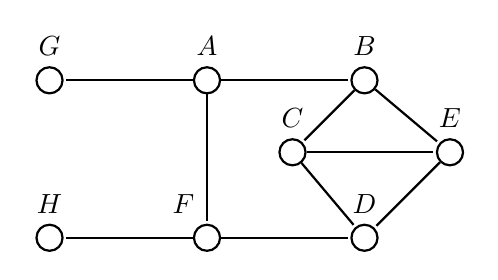
\begin{tikzpicture}[>=stealth',shorten >=1pt,auto,node distance=2cm,
		thick,main node/.style={circle,draw,font=\small},scale=0.5]
		
		\node[main node] (2) [label=$A$]{};
		\node[main node] (1) [left of=2] [label=$G$]{};                 
		\node[main node] (3) [right of=2] [label=$B$]{};
		\node[main node] (4) [below of=2] [label={[xshift=-0.3cm]$F$}]{};
		\node[main node] (5) [below left of=3, yshift=0.5cm, xshift=0.5cm] [label=$C$]{};
		\node[main node] (6) [right of=5] [label=$E$]{};
		\node[main node] (7) [below of=3] [label=$D$]{};
		\node[main node] (8) [left of=4] [label=$H$]{};
		
		\path[every node/.style={font=\sffamily\small,sloped,anchor=south,auto=false}]
		(2) edge node {} (1)
		(2) edge node {} (4)
		(2) edge node {} (3)
		(3) edge node {} (5)
		(3) edge node {} (6)
		(5) edge node {} (6)
		(5) edge node {} (7)
		(6) edge node {} (7)
		(4) edge node {} (7)
		(4) edge node {} (8);
		\end{tikzpicture}
		\caption{Example graph for the branch-and-bound \textsf{DSATUR} algorithm}\label{fig:8}
	\end{figure}
	
	\begin{figure*}[h]
		\centering
		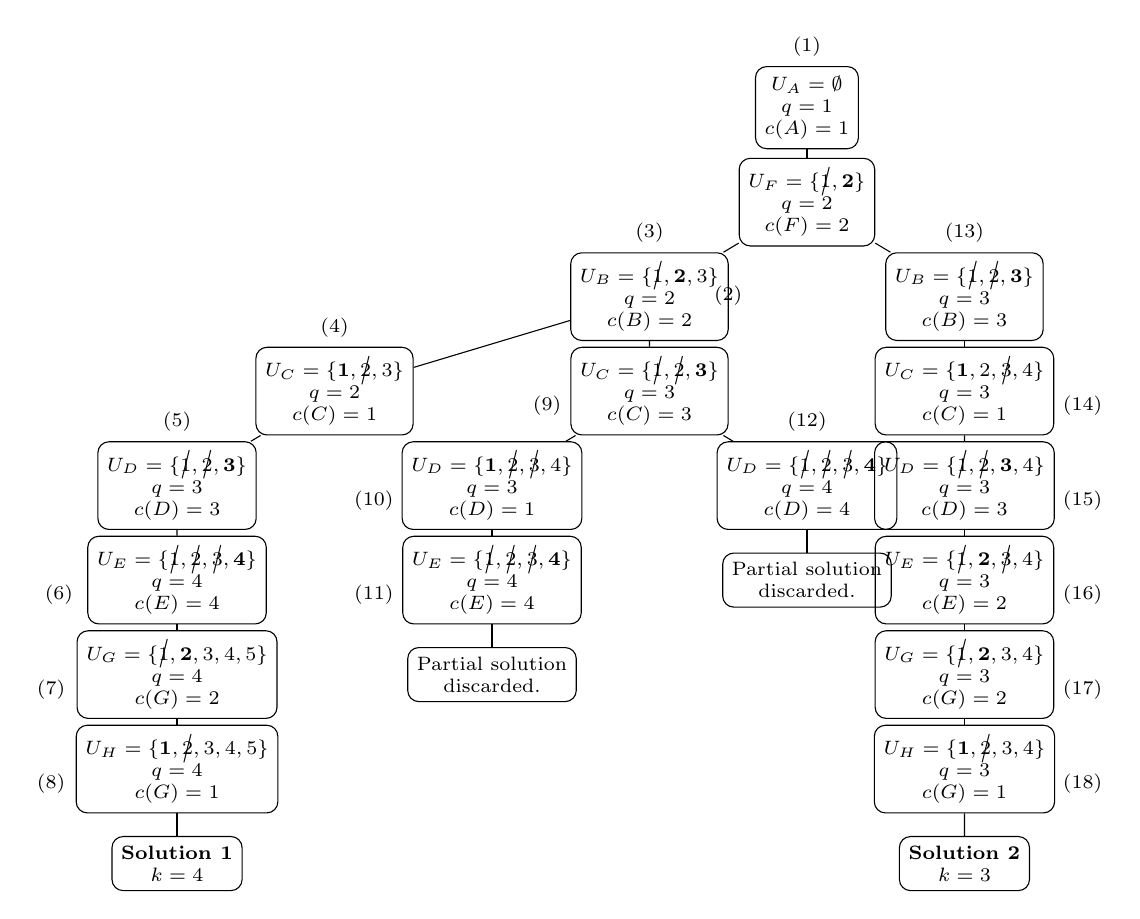
\begin{tikzpicture}[sibling distance=5cm,
		every node/.style = {shape=rectangle, rounded corners,
			draw, align=center, font=\scriptsize},scale=0.8]
		\node [label=(1)]{$U_A=\emptyset$\\$q=1$\\ $c(A) = 1$}
		child { node [label={[xshift=-1cm, yshift=-2cm](2)}]{$U_F=\{\cancel{1},\textbf{2}\}$\\$q=2$\\$c(F) = 2$}
			child { node [label=(3)]{$U_B=\{\cancel{1},\textbf{2},3\}$\\$q=2$\\$c(B) = 2$} 
				child { node [label=(4)]{$U_C=\{\textbf{1},\cancel{2},3\}$\\$q=2$\\$c(C) = 1$} 
					child { node [label=(5)]{$U_D=\{\cancel{1},\cancel{2},\textbf{3}\}$\\$q=3$\\$c(D) = 3$} 
						child { node [label={[xshift=-1.5cm,yshift=-1cm](6)}]{$U_E=\{\cancel{1},\cancel{2},\cancel{3},\textbf{4}\}$\\$q=4$\\$c(E) = 4$} 
							child { node [label={[xshift=-1.6cm,yshift=-1cm](7)}]{$U_G=\{\cancel{1},\textbf{2},3,4,5\}$\\$q=4$\\$c(G) = 2$} 
								child { node [label={[xshift=-1.6cm,yshift=-1cm](8)}]{$U_H=\{\textbf{1},\cancel{2},3,4,5\}$\\$q=4$\\$c(G) = 1$}
									% 
									child { node {\textbf{Solution 1}\\$k=4$}}} } } }  
					child[missing]{ node {} } }
				child { node [label={[xshift=-1.3cm,yshift=-1cm](9)}]{$U_C=\{\cancel{1},\cancel{2},\textbf{3}\}$\\$q=3$\\$c(C) = 3$} 
					child { node [label={[xshift=-1.5cm,yshift=-1cm](10)}]{$U_D=\{\textbf{1},\cancel{2},\cancel{3},4\}$\\$q=3$\\$c(D) = 1$} 
						child { node [label={[xshift=-1.5cm,yshift=-1cm](11)}]{$U_E=\{\cancel{1},\cancel{2},\cancel{3},\textbf{4}\}$\\$q=4$\\$c(E) = 4$} 
							child { node {Partial solution\\ discarded.} } } }
					child { node [label=(12)]{$U_D=\{\cancel{1},\cancel{2},\cancel{3},\textbf{4}\}$\\$q=4$\\$c(D) = 4$} 
						child { node {Partial solution\\ discarded.} } } }
				child[missing] {node {}} } 
			child { node [label=(13)]{$U_B=\{\cancel{1},\cancel{2},\textbf{3}\}$\\$q=3$\\$c(B) = 3$}
				child { node [label={[xshift=1.5cm,yshift=-1cm](14)}]{$U_C=\{\textbf{1},2,\cancel{3},4\}$\\$q=3$\\$c(C) = 1$} 
					child { node [label={[xshift=1.5cm,yshift=-1cm](15)}]{$U_D=\{\cancel{1},\cancel{2},\textbf{3},4\}$\\$q=3$\\$c(D) = 3$}
						child { node [label={[xshift=1.5cm,yshift=-1cm](16)}]{$U_E=\{\cancel{1},\textbf{2},\cancel{3},4\}$\\$q=3$\\$c(E) = 2$} 
							child { node [label={[xshift=1.5cm,yshift=-1cm](17)}]{$U_G=\{\cancel{1},\textbf{2},3,4\}$\\$q=3$\\$c(G) = 2$} 
								child { node [label={[xshift=1.5cm,yshift=-1cm](18)}]{$U_H=\{\textbf{1},\cancel{2},3,4\}$\\$q=3$\\$c(G) = 1$} 
									child { node {\textbf{Solution 2}\\$k = 3$} } } } } } } } }
		% 
		
		child[missing] { node {} };
		\end{tikzpicture}
		
		\caption{State space search tree of the branch-and-bound \textsf{DSATUR} on the graph of Figure~\ref{fig:8}}\label{fig:9}
	\end{figure*}
	
	The most recent adaptation of Brelaz's algorithm~\cite{Brelaz79} can
	be found in the work of Sewell~\cite{Sewell1996} and San Segundo~\cite{SanSegundo2012}. They proposed new tie breakers in the
	step of choosing the vertex with the greatest degree of
	saturation. 
	
	The algorithm of Sewell~\cite{Sewell1996} chooses the
	vertex that shares the greatest amount of available colors with its
	neighbors in the uncolored subgraph, while the algorithm of San Segundo~\cite{SanSegundo2012} chooses the vertex that shares the
	greatest amount of colors with the vertices that have the same
	greatest degree of saturation.
	Furini, Gabrel and Ternier\cite{Furini2017} also made an adaptation of Brelaz's
	algorithm, although their modification was done in the updating step of the global upper bound for the chromatic number.
	
	Tests of the algorithms of Brelaz~\cite{Brelaz79} and Sewell~\cite{Sewell1996} have been done by San Segundo~\cite{SanSegundo2012}. The algorithms were executed in random
	graphs with at most 80 vertices and in some DIMACS~\cite{dimacs} instances. The author
	concluded that the three algorithms have similar results, except in
	graphs of densities up to 0.7, which \cite{SanSegundo2012} is more efficient. In almost all DIMACS instances, San Segundo's algorithm ~\cite{SanSegundo2012} had the best performance.
	Results in~\cite{Furini2017} are similar to the ones in~\cite{SanSegundo2012}. For the random graphs instances, the algorithm of Furini, Gabrel and Ternier~\cite{Furini2017} had better results to graphs from 75 to 80 vertices, but the computational costs in relation to~\cite{SanSegundo2012} is small.
	
	%..............................................................................
	\subsection{Zykov's Algorithm}\label{sec:zykov}
	
	The algorithm of Zykov~\cite{Zykov1952} (Algorithms~\ref{alg:13} and~\ref{alg:14}~\cite{AraujoNetoGomes2014}) is based in his recurrence
	which states that, if $G$ is a graph and for any pair of vertices $x,y \in V(G)$ that do not share an
	edge, an optimal coloring of $G$ can either assign the same color to
	$x$ and $y$ or not (Theorem~\ref{teo:9}).
	
	In this section, we first show the basis of Zykov's algorithm, which
	he called \emph{a Zykov tree}. Then, we discuss about the analysis of
	the worst case of the algorithm (Theorem~\ref{teo:zyk}), based in~\cite{AraujoNetoGomes2014}, and some of
	the results found in the literature.
	
	
	\subsubsection{Zykov Trees}
	
	Zykov~\cite{Zykov1952} has stated we can obtain two new graphs from
	$G$, for a given pair of vertices $x,y \in V(G)$ that are not neighbors. One of
	these graphs will contract $x$ and $y$ into a single vertex, while the
	other will create an edge between $x$ and $y$. The chromatic
	number of $G$ corresponds to the minimum chromatic number of one of
	these graphs. In other words, an optimal coloring of the first graph
	assign the same color to $x$ and $y$, while an optimal coloring of the
	second graph assign different colors to $x$ and $y$.
	
	\begin{defin}
		For two vertices $x,y \in V(G)$ that do not share and edge, a
		\emph{contraction} in $G$ produces a new graph $G'_{xy}$ given by
		\begin{small}
		\begin{equation*}
		\begin{aligned}
		V(G_{xy}') &= V(G) \setminus \chaves{x,y} \cup \chaves{z}\\
		% \begin{equation*}
		E(G_{xy}') &= \left\{
		\begin{aligned}
		& \chaves{u,v} \in E(G) \text{ such that } x \notin \chaves{u,v} \text{ and } y \notin \chaves{u,v}\\
		& \cup \\
		& \chaves{u,z} \text{ such that } \chaves{u,x} \in E(G) \text{ or } \chaves{u,y} \in E(G)
		\end{aligned} \right\}
		% \end{equation*}\nonumber
		\end{aligned}
		\end{equation*}\nonumber
		\end{small}
		For two vertices $x,y \in V(G)$ that do not share and edge, an
		\emph{addition} in $G$ produces a new graph $G''_{xy}$ given by
		
		\begin{equation*}
		\begin{aligned}
		V(G_{xy}'') &= V(G)\\
		E(G_{xy}'') &= E(G) \cup \chaves{\chaves{x,y}}
		\end{aligned}
		\end{equation*}
	\end{defin}
	
	\begin{teor}\label{teo:9}
		The chromatic number of $G$ is given by the recurrence
		\begin{multline*}
		\chi(G) 
		=
		\Min{\chi(G_{xy}'),\chi(G_{xy}'')} \\
		\text{ such that } x,y \in V(G) \text{ and } \chaves{x,y} \notin E(G)
		\end{multline*}
	\end{teor}
	
	The recurrence of Theorem~\ref{teo:9} builds a binary tree called
	\emph{Zykov tree} where its leaf nodes are cliques and the chromatic
	number of the graph is given by the smallest clique of the tree.
	
	Zykov trees have exactly one branch formed only by contraction
	operations, where the size of the clique of this branch is an upper
	bound $q$ for the chromatic number. This bound is updated each time a better coloring than the current one is found. In a
	Branch-and-Bound version of Zykov's algorithm, operations
	of contractions and additions will happen only in graphs that do not
	have a $q$-clique on its structure. Figure~\ref{fig:13} shows an
	example of the Algorithms~\ref{alg:13} and~\ref{alg:14} on the graph represented in the tree's root.
	
	\begin{algorithm}[h]
		\SetAlgoNoLine
		\KwData{A graph $G$}
		\KwResult{The minimum value $q$}
		$n \gets |V(G)|$
		
		\If{$G$ is a complete graph}{
			$q \gets \Min{n,q}$
		}\ElseIf{$G$ does not have a $q$-clique}{
			Choose $x,y \in V(G)$ such that $\chaves{x,y} \notin E(G)$.
			
			$\text{Color}(G_{xy}')$ //vertex contraction
			
			$\text{Color}(G_{xy}'')$ //edge addition
		}
		\Return{$q$}
		\caption{$\textsc{Color($G$)}$}\label{alg:13}
	\end{algorithm}
	
	\begin{algorithm}[h]
		\SetAlgoNoLine
		\KwData{A graph $G$}
		\KwResult{The chromatic number of $G$}
		$n \gets |V(G)|$
		
		$\chi(G) \gets \text{ Color}(G)$               \\              
		\Return{$\chi(G)$}
		\caption{$\textsc{Zykov(G)}$}\label{alg:14}
	\end{algorithm}
	
	\begin{figure}[h]
		\centering
		\includegraphics[scale=0.275]{arvore_zykov2}
		\caption{Pruned Zykov tree}\label{fig:13}
	\end{figure}
	
	\begin{teor} An algorithm based on
		Zykov trees has complexity $\cO(2^{n^2})$ and space $\cO(n^2(n+m))$, if the input is a graph with $n$ vertices and $m$ edges.\label{teo:zyk}
	\end{teor}
	
	\begin{proof} The height of a Zykov tree is at most $\overline{m}$,
		which is the number of complementary edges so that the graph be
		complete. Each level $i$ of the tree has $2^i$ nodes, so the size of
		the tree is 
		
		\begin{equation*}
		\sum_{i=0}^{\overline{m}} 2^i 
		=
		\frac{2^{\overline{m}+1}-1}{2-1} = 2^{\bar{m}+1}-1 
		=
		2^{\frac{n(n-1)}{2}+1}-1
		\end{equation*}
		
		The amount of memory necessary in
		algorithms of this kind is $\cO(n^2(n+m))$, since the whole graph is stored on each level of the recursion.
	\end{proof}
	
	Corneil and Graham~\cite{CorneilGraham1973} adapted Zykov's algorithm to find the
	pair of vertices that are not neighbors in a $q$-cluster, which is a
	dense subgraph of $G$. Their algorithm uses an amount
	$\cO(n^3)$ of memory.
	
	McDiarmid~\cite{McDiarmid1979}, on the other hand, focused on doing a more
	detailed worst case analysis of Zykov's algorithms, concluding that
	this algorithms are not more efficient than the ones that are based on
	generating the maximal independent sets of a graph. He concluded that
	for almost all graphs, a Zykov tree has size $\cO(e^{cn
		\sqrt{\log n}})$, where $c$ is a constant $c>1$.
	
	%------------------------------------------------------------------------------
	\section{Integer Linear Programming Algorithms}\label{sec:lp}
	
	In this section, we present the algorithms that solve graph coloring
	instances as integer linear programs, which are based in the previous
	work of Mehrotra and Trick~\cite{Mehrotra95}. We first show some definitions of
	Linear Programming and formulations of the graph coloring problem as
	integer linear programs (ILP).
	
	Mehrotra and Trick~\cite{Mehrotra95} use the Branch-and-Price method, which combines the methods of Branch-and-Bound and Column Generation. We describe their algorithm and
	discuss about its most recent adaptations.
	
	%..............................................................................
	\subsection{Integer Linear Programming}
	
	When we have an optimization problem where a linear function subject
	to a set of linear constraints is given, then we have a \emph{linear
		program}. When the objective is to find the smallest value for the
	function, then we have a linear minimization program.
	
	Let $n,m \in \mathbb{N}^*$, $A \in \mathbb{Q}^{n \times m}$ and the arrays $c \in
	\mathbb{Q}^n$, $x \in \mathbb{Q}^n_{+}$ and $b \in \mathbb{Q}^m$
	represented as columns. $c^T$ denotes the array $c$ transposed. The canonical and the standard formulations of a linear program are
	defined below.
	
	\begin{defin} The canonical formulation of a linear program, defined
		by $A$, $b$ and $c$, is given by
		
		\begin{equation*}
		\begin{aligned}[c] \text{Minimize } & z = c^{T}x\\ \text{subject to }&
		Ax \geq b\\ & x \geq 0
		\end{aligned}
		\end{equation*}\label{def:1a}
	\end{defin}
	
	\begin{defin} The standard formulation of a linear program, defined by
		$A$, $b$ and $c$, is given by
		
		\begin{equation*}
		\begin{aligned}[c] \text{Minimize } & z = c^{T}x\\ \text{subject to }&
		Ax = b\\ & x \geq 0
		\end{aligned}
		\end{equation*}\label{def:1b}
	\end{defin}
	
	A canonical formulation can be converted into a standard one with the
	addition of slack variables. More details about it can be checked in \cite{MatousekGaertner07}.
	
	When we have a linear program where the values of $x$ are integer,
	then we have an \emph{integer linear program}. The value of the
	non-integer optimal solution of a linear program is a lower bound for
	its integer optimal solution value, and the difference between these
	two values is called integrality gap. Solving a linear program is a
	polynomial problem, and the most known algorithm that solves a linear
	program is the Simplex Algorithm~\cite{Dantzig1963}. On the other hand,
	solving an integer linear program is a $\NP$-Hard problem,
	since a Branch-and-Bound algorithm combined to the Simplex is
	necessary to solve it optimally~\cite{PapadimitriouSteiglitz98}.
	
	
	\subsubsection{ILP formulations for the graph coloring problem}
	
	For a graph $G$ where $n = |V(G)|$ and $m = |E(G)|$, a first formulation for the graph
	coloring problem as an ILP is given by Formulation~\eqref{pl1}, defined by the equations~\eqref{pl1:a},~\eqref{pl1:b},~\eqref{pl1:c},~\eqref{pl1:d} and~\eqref{pl1:e}.
	
	\begin{subequations}\label{pl1}
		\begin{align}
		\text{Minimize}  & \displaystyle\sum\limits_{j=1}^{n} x_{j} & \label{pl1:a}\ \\
		\text{subject to:}& \displaystyle\sum\limits_{j=1}^{n} y_{vj} = 1,  &&\text{ for all } v \in V(G) \nonumber \\
		&&&\text{ and } j \in \chaves{1, \ldots,n}\label{pl1:b}\ \\
		&y_{vj} + y_{uj} \leq x_j, &&\text{ for all } \chaves{v,u} \in E(G) \nonumber\\      
		&&&\text{ and } j \in \chaves{1, \ldots,n}\label{pl1:c}\ \\
		&y_{vj} \in \chaves{0,1}, &&\text{ for all } v \in V(G)\nonumber\\
		&&&\text{ and } j \in \chaves{1, \ldots,n}\label{pl1:d}\ \\
		&x_{j} \in \chaves{0,1}, &&\text{ for all } j \in \chaves{1, \ldots,n}\label{pl1:e}\
		\end{align}
	\end{subequations}
	
	In this formulation, there is one binary variable $x_j$ for each color
	$j$ indicating if that color is part of a solution or not. Each
	variable $y_{vj}$ indicates if the color $j$ is assigned to the vertex
	$v$. The objective function describes a minimization integer linear
	program, since an optimal solution has the minimum number of colors assigned to the vertices. The set of constraints in~\eqref{pl1:b} describes that
	a vertex can only have one color assigned to it. Each constraint in~\eqref{pl1:c} describes that vertices that share an edge cannot have the
	same color.
	
	Formulation~\eqref{pl1} has a polynomial amount of constraints and variables,
	but it generates a factorial set of symmetric solutions. That is, a solution is symmetric when it can be represented as a combination of different
	valuations. It turns the state space search tree of the Branch-and-Bound algorithm
	too large, as Lewis~\cite{Lewis2015} exposes. 
	
	Let the equations~\eqref{pl2:a},~\eqref{pl2:b} and~\eqref{pl2:c} be the Formulation~\eqref{pl2}, proposed by Mehrotra and Trick~\cite{Mehrotra95}.
	
	\begin{subequations}\label{pl2}
		\begin{align}
		\text{Minimize } & \displaystyle\sum_{S \in \boldsymbol{S}} x_S & \label{pl2:a}\ \\
		\text{subject to: } & \displaystyle\sum_{\chaves{S:v \in S}} x_S \geq 1, &&\text{ for all } v \in V(G) \label{pl2:b}\ \\
		& x_S \in \chaves{0,1}, && \text{ for all } S \in \textbf{S} \label{pl2:c}\
		\end{align}
	\end{subequations}
	
	In Formulation~\eqref{pl2}, \textbf{S} is the set of the maximal independent
	sets of a graph and the binary variable $x_S$ indicates whether a set
	$S \in \textbf{S}$ is part of a solution or not. The objective function
	in~\eqref{pl2:a} indicates that the chromatic number of a graph
	corresponds to the minimum set cover. Each constraint in~\eqref{pl2:b}
	indicates that each vertex $v$ must be contained in at least one
	maximal independent set $S$. Although this formulation has an
	exponential number of variables, the problem of symmetry is avoided.
	
	\paragraph{Fractional coloring}
	
	A non-integer optimal solution of the Formulation~\eqref{pl2} gives a
	fractional coloring of $G$. That is, since each maximal independent
	set represents a color, then each vertex will receive a set of colors
	instead of just one in a fractional coloring. Besides, the sets of
	vertices that share and edge will be disjoint. The value of an optimal
	fractional coloring is called \emph{fractional chromatic number}, denoted by
	$\chi_f(G)$.
	
	For example, let $S_1$ and $S_2$ be two maximal independent sets and
	let $x_{S_1}+x_{S_2} \geq 1$ be the constraint for a vertex $v \in
	V(G)$. If $x_{S_1}$ and $x_{S_2}$ have values 0.5, for example, then
	it means these colors contributes to 0.5 each in the fractional
	chromatic number, and the vertex $v$ has both $S_1$ and $S_2$
	assigned to it.
	
	The integrality gap between $\chi_f(G)$ and $\chi(G)$ is $\cO(\log
	n)$\linebreak~\cite{Lund1994}, although finding $\chi_f(G)$ is also an $\NP$-Hard
	problem.
	
	%..............................................................................
	\subsection{Column Generation}
	
	Sometimes we cannot escape the fact that some formulations have a
	large set of variables, such as the Formulation~\eqref{pl2}. They are
	still used in literature because they may avoid the problem of
	symmetry in solutions~\cite{Barnhart98}. One of the problems of this
	kind of formulation is that many variables may not be in the optimal
	solution. A way around it is to start solving the instance with a
	small set of the variables and add the others as necessary.
	
	The Column Generation method uses this approach to solve linear programs with a large set
	of variables. The \emph{column} in the method's name refers to
	the Simplex algorithm in tableau format, where each column is
	associated to a variable.
	
	A Column Generation based algorithm decomposes the linear program in
	two, named Master Problem and Pricing Problem. The first one is a more
	restricted reformulation of the original linear program, while the
	second one is the linear program that determines the variables that
	will be gradually added to the Master Problem. Both of the problems
	can be obtained by the Dantzig-Wolfe Linear Decomposition~\cite{Dantzig1963}. A description to this decomposition is given by Andrade, Miyazawa and Xavier~\cite{Andrade2006}.
	
	For a given linear program in the standard form, the main idea of a
	Column Generation based algorithm is to find an initial set of the
	variables such that the Master Problem has at least one viable
	solution from this set. The Master Problem is solved with this set
	using the Simplex Algorithm. This is called the Restricted Master
	Problem (RMP).
	
	Before showing a general description to a Column Generation algorithm,
	we review the pricing step of the Simplex Algorithm, since the Pricing
	Problem comes from this stage.
	
	The solution found by the Simplex Algorithm separates the indices of
	the variables in two sets $B$ and $N$. The set $B$ has dimension $m$
	and the variables associated to this set is called the basic variables
	(or the basis $B$). The set $N$ is the set of the indices that are not
	in $B$, and the variables associated to it are called the non-basic
	ones. We denote the set of the basic and non-basic variables as $x_B$
	and $x_N$, respectively. We also denote the sets of the costs of the
	basic and non-basic variables as $c_B$ and $c_N$, respectively. Each
	variable in $x_B$ has value greater or equal than 0 and every variable
	in $x_N$ is equal to 0.
	
	The matrix $A$ can be rewritten as $A = [A_B|A_N]$, where $A_B = {\chaves{A_i}}_{i \in B}$, $A_N = {\chaves{A_i}}_{i \in N}$ and $A_B$ is
	non-singular. We obtain the following equivalence:
	\begin{equation*}
	Ax = b \iff A_{B}x_{B} + A_{N}x_{N} = b \iff
	\end{equation*}
	\begin{small}
	\begin{equation*}
	\iff A_{B}^{-1} A_{B}x_{B} + A_{B}^{-1} A_{N}x_{N} = A_{B}^{-1}b \iff x_{B} = A_{B}^{-1}b - A_{B}^{-1}A_{N}x_{N}
	\end{equation*}
	\end{small}
	Rewriting the objective function substituting $x_B$ for the expression
	found above, we have
	
	\begin{multline*}
	z = c_{B}^{T}x_{B} + c_{N}^{T}x_{N} = c_{B}^{T}(A_{B}^{-1}b - A_{B}^{-1}A_{N}x_{N}) + c_{N}^{T}x_{N} \\= c_{B}^{T}A_{B}^{-1}b + x_{N}(c_{N}^{T} - c_{B}^{T}A_{B}^{-1}A_{N})
	\end{multline*}
	
	The pricing step of the Simplex Algorithm, then, will find the
	non-basic variable that has the minimum reduced cost to enter the
	basis, that is, the minimum negative value of $c_{N}^{T} -
	c_{B}^{T}A_{B}^{-1}A_{N}$. Only the non-basic variables are examined since the
	basic variables has its reduced cost equals to zero. We denote
	$A_B^{-1}$ as $\lambda$.
	
	For a given linear program that has an optimal solution, let $n$ be
	its number of variables. The Column Generation is generically
	described as follows (Algorithm~\ref{alg:8}).
	
	\begin{algorithm*}[htpb]
		\SetAlgoNoLine
		\KwData{The $m \times n$ matrix $A$ and the arrays $b$ and $c$ of dimensions $m$ and $n$, respectively.}
		\KwResult{The optimal solution of the linear program defined by $A$, $b$ and $c$, such that $Ax = b$ and $c^{T}x$ is minimum.}
		
		Let $P$ be the linear program formulated from $A$, $b$ and $c$.\\[5pt]
		
		Get the Master Problem of $P$ from the Dantzig-Wolfe linear decomposition.\\[5pt]
		
		Get the Restricted Master Problem RMP.\\[5pt]
		
		\Do{there is $\overline{c}_i < 0$ in $\overline{c}$}{
			\justifying 
			Solve the RMP by the Simplex Algorithm.\\[5pt]
			
			Define the set of non-basic variables as the set that has the non-basic variables found in the non-integer solution of the RMP and the variables that are not in the RMP yet. Formulate the Pricing Problem (PP) from the pricing step of the Simplex Algorithm, that is,
			\begin{equation*}
			\overline{c} = c_N^T - \lambda^T{A}_N
			\end{equation*}
			\begin{equation*}
			\overline{c}_i \in \overline{c} \text{ such that } \overline{c}_i \text{ is minimum and } i \in N
			\end{equation*}
			Solve the PP\@. If $\overline{c}_i < 0$, then add the variable found in PP to the RMP\@. Otherwise, the solution of the RMP is also an optimal solution to the linear program given as input.\\[5pt]
		}
		\Return{$x$}
		\caption{\textsc{Column Generation}}\label{alg:8}
	\end{algorithm*}
	
	A Branch-and-Bound algorithm that uses the Column Generation method is
	called a Branch-and-Price algorithm, and it is illustrated in the
	Figure~\ref{fig:7}. When a branching step occurs, it means that
	constraints are added to a linear program to force the value of a
	variable to be integer (details can be checked in~\cite{MatousekGaertner07}). In the Figure~\ref{fig:7}, $X$ is the set of the
	linear programs that are in the state space search tree to be solved.
	
	\begin{figure*}[htpb]
		%\includegraphics[scale=0.4]{flow}
		%\begin{comment}
		\centering
		
		\tikzstyle{decision} = [diamond, draw, text width=4.5em, text centered, node distance=3cm, inner sep=0pt]
		\tikzstyle{block} = [rectangle, draw, text width=21em, text centered, rounded corners, minimum height=2em]
		\tikzstyle{block2} = [rectangle, draw, text width=5em, text centered, rounded corners, minimum height=2em]
		\tikzstyle{block3} = [rectangle, draw, text width=20em, text justified, rounded corners, minimum height=2em]
		\tikzstyle{line} = [draw, -latex']
		\tikzstyle{cloud} = [draw, ellipse, node distance=3cm, minimum height=2em]
		
		\begin{tikzpicture}[node distance = 2cm, auto]
		% Place nodes
		\node [block] (init) {{\bf Input:} Integer Linear Program};
		\node [block, below of=init] (master) {Formulate the Master Problem by the Dantzig-Wolfe linear decomposition};
		\node [block, below of=master,node distance=2cm] (restrito) {Get the initial set of variables to constitute the Restricted Master Problem (RMP) by an heuristic, for example};
		\node [block, below of=restrito] (solucao) {Get the non-integer solution of the RMP};
		\node [block, below of=solucao] (sgc) {Formulate and solve the pricing problem};
		\node [block, below of=sgc] (reduzido) {Is there a reduced cost variable?};
		\node [block2, left of=sgc, node distance=7cm] (add) {Add the new variable to the RMP};
		\node [block, below of=reduzido] (fac) {Is the solution viable?};
		\node [block, below of=fac] (integral) {Is the solution integer?};
		\node [block3, below of=integral] (ram) {Branch the current instance and add the new instances to the $X$};
		\node [block2, left of=ram, node distance=7cm] (sub) {Is $X$ empty?};
		\node [block2, above of=sub, node distance=4cm] (pare) {{\bf Output:} An optimal solution, if possible.};       
		\node [block, below of=ram] (selec) {Select an instance of $X$};
		
		% Draw edges
		\path [line] (init) -- (master);
		\path [line] (master) -- (restrito);
		\path [line] (restrito) -- (solucao);
		\path [line] (solucao) -- (sgc);
		\path [line] (sgc) -- (reduzido);
		\path [line] (reduzido) -| node [very near start] {Yes} (add);
		\path [line] (reduzido) -- node [near start] {No} (fac);
		\path [line] (fac) -- node {Yes} (integral);
		\path [line] (add) |- (solucao);
		\path [line] (integral) -- +(-4.5,0) -- node [near start] {Yes} (sub);
		\path [line] (sub) -- node [near start] {Yes} (pare);
		\path [line] (integral) -- node [near start] {No} (ram);
		\path [line] (sub) |- node [near start] {No} (selec);
		\path [line] (selec) -- +(5,0) -- +(5,12) -- +(3.8,12) (solucao);
		\path [line] (fac) -- +(-4.5,0) -- node [very near start] {No} (sub);
		\path [line] (ram) -- (sub);
		\end{tikzpicture}
		%\end{comment}
		
		\captionof{figure}{Simplified flowchart of a Branch-and-Price algorithm}\label{fig:7}
	\end{figure*}
	
	%..............................................................................
	\subsection{Mehrotra and Trick Algorithm}
	
	The first exact algorithm for the graph coloring that use the
	Branch-and-Price method was proposed by Mehrotra and Trick~\cite{Mehrotra95}. The Master Problem is composed by Formulation~\eqref{pl2} without the integrality constraints.
	
	The Restricted Master Problem is described in Formulation \eqref{pl3}, which is defined by the equations \eqref{pl3:a} and \eqref{pl3:b}. To get the initial set of variables $\overline{\textbf{S}} \in
	\textbf{S}$ for the Restricted Master Problem, the authors use an heuristic procedure for the Maximum Weighted Independent
	Set (MWIS) problem. We describe this heuristic in Algorithm~\ref{alg:9}. We show that the Pricing Problem of their algorithm
	is equivalent to solve the Maximum Weighted Independent Set problem,
	in fact. We finally describe the rule proposed by the authors in the branching step of the algorithm. The most recent adaptations of Mehrotra and Trick~\cite{Mehrotra95} can be found in the work of Malaguti and Toth~\cite{Malaguti2010} and Gualandi and Malucelli~\cite{Gualandi2010}.
	
	\subsubsection{The Pricing Problem}
	
	As we mentioned before, Mehrotra and Trick~\cite{Mehrotra95} find the initial set
	of variables to the Restricted Master Problem, defined as follows.
	
	\begin{subequations}\label{pl3}
		\begin{align}
		\text{Minimize } & \displaystyle\sum_{s \in \boldsymbol{\overline{S}}} x_S &\label{pl3:a}\ \\
		\text{subject to: } & \displaystyle\sum_{\chaves{S:v \in S}} x_S \geq 1, &&\text{ for all } v \in V(G)\label{pl3:b}\ \\
		& x_S \geq 0, && \text{ for all } S \in \overline{\textbf{S}}\nonumber
		\end{align}
	\end{subequations}
	
	The authors use an heuristic to the Maximum Weighted Independent Set problem
	(MWIS), that we define below. The heuristic is described in Algorithm~\ref{alg:9}.
	
	\begin{samepage}
		\begin{framed}
			\textbf{Maximum Weighted Independent Set (MWIS)}\\
			\emph{Input}: a graph $G$ and a function $w: V(G) \rightarrow \mathbb{Q}$ such that $w(v)$ is named \emph{weight} of the vertex $v \in V(G)$. \\
			\emph{Answer}: a maximum weighted independent set, that is, an independent set $I \subseteq V(G)$ such that $\displaystyle\sum_{v \in I} w(v)$ is maximum.
		\end{framed}
	\end{samepage}
	
	\begin{algorithm}[h]
		\SetAlgoNoLine
		\KwData{A graph $G$}
		\KwResult{A maximal weighted independent set}
		$I \gets \emptyset$\\
		\Do{$V(G) \neq \emptyset$}{
			\justifying 
			Choose a vertex $v \in V(G)$ of maximum weight.
			
			Add $v$ to $I$.
			
			Remove $N_G(v)$ from $V(G)$.
		}
		\Return{$I$}
		\caption{\textsc{Greedy heuristic for the $MWIS(G)$}}\label{alg:9}
	\end{algorithm}
	
	%This happens because the Pricing Problem searches for the non-basic variable with minimum reduced cost among the variables that are non-basic in the RMP and the ones that are not in the RMP yet.
	
	As we mentioned before, the Pricing Problem is obtained by the pricing
	step of the Simplex Algorithm, that is, $$\Min{c_N^{T} - \lambda^{T}A_{N}}\text{.}$$ More details of the relation between the dual and the pricing problems can be checked in~\cite{desaulniers2006}.
	
	In the Master Problem defined in Formulation~\eqref{pl2}, each coefficient in $c_N^T$ has value 1 and each
	variable is associated to a column of $A_N$, which describes an
	independent set $S$ that is represented as an array $z \in
	{\chaves{0,1}}^n$. Each row of the Master Problem is associated to a vertex
	$v \in V(G)$, so we can denote $\lambda_v$ as the dual value obtained by $v$
	in the non-integer solution of the RMP\@. Hence, we have that the
	Pricing Problem corresponds to $\Min{1-\lambda^{T}z}$, that is, 
	
	\begin{equation*}
	\Min{
		1-\displaystyle\sum\limits_{v \in V(G)} \lambda_v z_v} \equiv 1 -
	\Max{\displaystyle\sum\limits_{v \in V(G)} \lambda_v z_v}
	\end{equation*}
	
	Formulation \eqref{pl4}, defined by \eqref{pl4:a} and \eqref{pl4:b}, describes the Pricing Problem, which is in fact the Maximum Weighted Independent Set problem. If the optimal solution of this formulation is greater than 1, then the
	independent set $S$ that will be added to the RMP is constituted by
	each vertex $v$ where $z_v = 1$, that is, $S = \chaves{v \in V(G) \text{ such
			that } z_v = 1}$. Otherwise, there is no independent set that can
	improve the current solution of the Master Problem.
	
	\begin{subequations}\label{pl4}
		\begin{align}
		\text{Maximize}  & \displaystyle\sum\limits_{v \in V(G)} \lambda_v z_v & \label{pl4:a}\ \\
		&z_u + z_v \leq 1, &&\text{ for all } \chaves{u,v} \in E(G) \label{pl4:b}\ \\        
		&z_v \in \chaves{0,1}, &&\text{ for all } v \in V(G)\nonumber
		\end{align}
	\end{subequations}
	
	\subsubsection{The Branching Rule}
	
	The branching step follows the Zykov rule described in Subsection~\ref{sec:zykov}. For an instance of the state space search tree, let
	$S_1$ and $S_2$ be two maximal independent sets and $x_{S_1}$ and
	$x_{S_2}$ the variables associated to these sets, such that at least
	one of them got a non-integer value. Since the non-integer optimal
	solution of the Master Problem represents a fractional coloring, then
	there are two vertices $u,v \in V(G)$ such that, without loss of
	generality, $u \in S_1 \cap S_2$ and $v \in S_1 \setminus S_2$. It means that whether
	$u$ can receive the same color as the vertices in $S_1$ (and so does
	$v$) or it can receive the same color as the vertices of $S_2$. Then,
	one of the new instances to be added to the state space search tree
	will have a constraint where $u$ and $v$ are contracted in one vertex,
	while the other new instance will have a constraint where $u$ and $v$
	have an edge between them. In fact, the constraint will be updated, so it is not necessary to create new constraints to the new instances.
	
	\subsubsection{Further Work}
		
	Mehrotra and Trick~\cite{Mehrotra95} observe that improvements in their method can
	be done in the algorithm that solves the MWIS problem. In their work,
	they propose a recurrence where given a graph $G$ and a vertex $v \in
	V(G)$, the MWIS can either exclude $v$ or have $v$ and the vertices
	that are not neighbors of $v$, that is, 
	\begin{equation*}
	MWIS(G) =
	\Max{MWIS(G-v),MWIS(G[\{v\} \cup \overline{N}_G(v)])}
	\end{equation*}
	The most recent adaptations of their algorithm can be found in the works of Malaguti and Toth~\cite{Malaguti2010} and Gualandi and Malucelli~\cite{Gualandi2010}. The first one
	uses a tabu search based heuristic to find the MWIS in the pricing
	step. This heuristic is executed for a fixed number of iterations. If
	this number is attained and a column were not found, then the instance
	of the MWIS is solved as a linear program. Gualandi and Malucelli~\cite{Gualandi2010},
	on the other hand, use Constraint Programming in the pricing step.
	
	San Segundo~\cite{SanSegundo2012} and Furini, Gabrel and Ternier~\cite{Furini2017} compare their
	algorithms with the implementation of Malaguti and Toth~\cite{Malaguti2010}, and
	they conclude that the Branch-and-Price based algorithms are currently
	the most efficient ones for hard DIMACS instances, while the
	algorithms based on the exact version of the \textsf{DSATUR} are the best ones
	for random graphs with 60 to 80 vertices and densities between 0.1 and
	0.9.
	
	%------------------------------------------------------------------------------
	\section{Conclusion}\label{sec:conclusion}
	

	
	
	In this work, we presented the most recent exact algorithms for the
	graph coloring problem, which are the ones based in Dynamic
	Programming, Branch-and-Bound and Integer Linear Programming. The
	algorithms of the first group have an worst case analysis, while the
	other ones have only an experimental analysis. We briefly
	introduce the information required to the comprehension of the exact
	algorithms that solve graph coloring instances. We also observe that
	the algorithms based in Branch-and-Price and Branch-and-Bound \textsf{DSATUR}
	are the most promising for the graph coloring problem, where the most
	recent are based in the previous work of Mehrotra and Trick~\cite{Mehrotra95} for
	the first group and Brelaz~\cite{Brelaz79} for the second group. Tables~\ref{tab:conc} and~\ref{tab:conc2} show an overview of the algorithms presented in this work.
	

	
	We observe that besides the differences between the exact approaches, they show similarities that are not always
	clear to the researcher. The algorithm proposed by Eppstein~\cite{Eppstein03} for the optimal coloring problem, for example, can be actually extended to the algorithms of Lawler~\cite{Lawler76} and Byskov~\cite{Byskov03}, without affecting the result of the respective analyses. Similarities between different paradigms also can be found. The Zykov's recurrence, for example, is much
	less efficient than other approaches, but it is useful in the
	branching step of Branch-and-Price algorithms, since this kind of rule does not change the original structure of the problem. Besides, we can cite the \textsf{DSATUR} procedure either as a simple heuristic for finding an initial upper bound for the chromatic number of a graph, or as a good exact algorithm for random graphs.
	
	
	\begin{table}[!h]
		\centering
				\caption{\label{tab:conc} Overview of the Dynamic Programming based algorithms}
		\begin{adjustbox}{width=\columnwidth}
		\begin{tabular}{|c|c|c|c|}
			\toprule
			\small
			\textbf{Algorithm}               & \textbf{Problem} & \textbf{Results}                      & \textbf{Space}                     \\ \midrule
			Lawler (1976)                    & Chromatic number  & $\cO(2.4423^n)$                  & $\Theta(2^n)$                       \\ \midrule
			\multirow{2}{*}{Eppstein (2003)} & Chromatic number  & \multirow{2}{*}{$\cO(2.4150^n)$} & \multirow{4}{*}{$\cO(2^n)$} \\ \cline{2-2}
			& Optimal coloring   &                                          &                                     \\ \cline{1-3}
			\multirow{2}{*}{Byskov (2004)}   & Chromatic number  & \multirow{2}{*}{$\cO(2.4023^n)$} &                                     \\ \cline{2-2}
			& Optimal coloring   &                                          &                                     \\ \midrule
			Bodlaender \& Kratsch (2006)     & Chromatic number  & $\cO(5.283^n)$                   & $\cO(n \log n)$             \\ \bottomrule
		\end{tabular}
		\end{adjustbox}
		
	\end{table}
	
	\begin{table*}[!htb] 
		\centering
				\caption{\label{tab:conc2} Overview of the Branch-and-Bound and ILP based algorithms}
		\begin{tabular}{|p{2cm}|p{2cm}|p{2cm}|p{3.5cm}|p{2.1cm}|}
			\toprule
			\textbf{Design Paradigm}                    & \textbf{Method}                               & \textbf{Algorithm}                                  & \textbf{Results}                                                                                                                                                                                                                                                                   & \textbf{Type of instance}          \\ \midrule
			\multirow{8}{*}{}           & Backtracking                                  & Brown (1972)                                        & \multirow{2}{*}{}                                                                                                                                                                           & Random graphs                      \\ \cline{2-3} \cline{5-5} 
			& \multirow{5}{*}{} & Sewell (1998)                                       & Sewell's algorithm is more efficient than Brown's for graphs with more than 60 vertices.                                                                                                                                                                                                                                                                                  & Random graphs and DIMACS instances \\ \cline{3-5} Branch-and-Bound
			& Exact \textsf{DSATUR} (Brélaz (1979))                                              & \multirow{2}{*}{}                     & More efficient than Sewell's in dense graphs (density up to 0.7).                                                                                                                                                                                                                  & Random graphs                      \\ \cline{4-5} 
			&                                               & San Segundo (2012)                                                   & San Segundo's algorithm is more efficient than Sewell's in almost all instances.                                                                                                                                                                                                        & DIMACS instances                   \\ \cline{3-5} 
			&                                               & \multirow{2}{*}{} & Their algorithm is more efficient than San Segundo's for dense graphs (density from 0.7 to 0.9) and number of vertices from 75 to 80, but the computational cost difference is small. Their algorithm is also more efficient than the ILP algorithms in this type of instance. & Random graphs                      \\ \cline{4-5} 
			&                                               &           Furini, Gabrel and Ternier (2017)                                          & Similar results to San Segundo's algorithm.                                                                                                                                                                                                                                             & DIMACS instances                   \\ \cline{2-5} 
			& \multirow{2}{*}{Zykov trees}                  & Corneil e Graham (1973)                             & Storage bounded in $\cO(n^3)$.                                                                                                                                                                                                                                              & Random graphs                      \\ \cline{3-5} 
			&                                               & McDiarmid (1979)                                    & Analytical results. For almost all graphs, a Zykov tree has size $\cO(e^{c}n\sqrt{\log n})$.                                                                                                                                                                                  & ---                                  \\ \midrule
			\multirow{3}{*}{} & Branch-and-Price                              & Mehrotra and Trick (1995)                           & \multirow{3}{*}{}                                                                                                                                                                        & \multirow{3}{*}{}  \\ \cline{2-3} Integer Linear Programming
			& Branch-and-Price and Tabu Search   & Malaguti and Toth (2011)                            & More efficient results for these instances in relation to the Branch-and-Bound algorithms.                                                                                                                                                                                                                                                                                    &   DIMACS instances                                    \\ \cline{2-3}
			& Branch-and-Price and Constraint Programming & Gualandi and Malucelli (2012)                       &                                                                                                                                                                                                                                                                                    &                                \\ \bottomrule
		\end{tabular}
		
	\end{table*}
    \pagebreak
	\section*{Acknowledgements}
	
	This work was partially funded by \textsf{CNPq} (Proc. 428941/2016-8) 
	and \textsf{CAPES}.
		
	\section*{Author contributions}
	
	This paper is an abridged version of the first author's Master Dissertation \cite{Lima17} which was advised by the second author.
	
	
	%\newpage
	%----------------------------------------------------------------------------------------
	%       REFERENCE LIST
	%----------------------------------------------------------------------------------------
	
	\phantomsection
	
	
	\makeatletter
	\renewcommand\@biblabel[1]{{\parbox{0.7cm}{[#1]}}}
	\makeatother
	% References
	\renewcommand{\refname}{References}
	\bibliography{sample}
	
	
	
	
	
	\balance
\end{document}